\documentclass[a4paper,14pt]{article}

\usepackage{extsizes} % Возможность сделать 14-й шрифт

% Пакеты
\usepackage[warn]{mathtext}
\usepackage[utf8]{inputenc} 		% Кодировка исходного текста
\usepackage[english]{babel} % Локализация и переносы
\usepackage{caption}
\usepackage{listings}
\usepackage{amsmath,amsfonts,amssymb,amsthm,mathtools}
\usepackage{breqn}
\usepackage{wasysym}
\usepackage{float}					% "Плавающие" картинки
\usepackage{wrapfig}				% Обтекание фигур (таблиц, картинок)
\usepackage{lscape}
\usepackage{xcolor}
\usepackage{fancyhdr} 				% Загрузим пакет
\usepackage{dsfont}					% Для стрелочек и других матсимволов
\usepackage{multicol}				% Для "столбиков"
\usepackage[normalem]{ulem}
\usepackage{pdfpages}
\usepackage{graphicx}				% Вставка картинок правильная
\graphicspath{{pictures/}, {images/}, {}}
\DeclareGraphicsExtensions{.pdf,.png,.jpg}
\usepackage{pdfpages}

%Задаем ссылки
\usepackage{hyperref}
\hypersetup{
colorlinks=true,
linkcolor=red,
filecolor=magenta,
urlcolor=blue
}

% Задаем поля
\usepackage{geometry} 
\geometry{top=20mm}
\geometry{bottom=20mm}
\geometry{left=15mm}
\geometry{right=15mm}
\usepackage{extsizes}                   % Возможность сделать 14-й шрифт

\setcounter{section}{0}

%%%Библиотеки
%\usepackage{indentfirst}


%%% DRAGON STUFF
\usepackage{scalerel}

\DeclareMathOperator*{\myint}{\ThisStyle{\rotatebox{25}{$\SavedStyle\!\int\!\!\!$}}}

\DeclareMathOperator*{\myoint}{\ThisStyle{\rotatebox{25}{$\SavedStyle\!\oint\!\!\!$}}}
%%% END 

%%%Конец библиотек

%%%Настройка ссылок
\hypersetup
{
colorlinks=true,
linkcolor=blue,
filecolor=magenta,
urlcolor=blue
}
%%%Конец настройки ссылок


%%%Настройка колонтитулы
\pagestyle{fancy}

\fancyhead[L]{Homework}
\fancyhead[C]{Optimization}
%\fancyhead[R]{
\includegraphics[scale=0.14]{rus_mipt_logo.png}}
%\fancyfoot[L]{
\includegraphics[scale=0.025]{fupm.jpg}}
\fancyfoot[C]{\thepage}
\fancyfoot[R]{Kreinin Matvei, B05-003}
%%%конец настройки колонтитулы

\begin{document}
 \begin{center}
	\hfill \break
	\hfill \break	
	FEDERAL STATE AUTONOMOUS \\
    EDUCATIONAL INSTITUTION OF HIGHER EDUCATION \\
    MOSCOW INSTITUTE OF PHYSICS AND TECHNOLOGY \\
    (STATE UNIVERSITY) \\
    PHYSTECH-SCHOOL OF APPLIED MATHEMATICS AND COMPUTER SCIENCE\\

	\hfill \break

	Homework.
	
	\vspace{7em}
	
	\vspace{7em}
	\large{\textbf{<<Optimization>>}}\\

\end{center}

\vspace{13em}

\begin{flushright}
	\normalsize{3-rd year student, group B05-003}\\
	\normalsize{\textbf{Kreinin Matvei}}\\
\end{flushright}

%\vspace{\fill}

\begin{center}
	\normalsize{\textbf{Moscow, 2022}}
\end{center}


\thispagestyle{empty}
\setcounter{page}{0}


 %\Large \textbf{I need to do:  3.2, 3.5(B)}\newline \textbf{It's only 1.5 problems...}
 \normalsize
 
 \tableofcontents
 
 \section{Matrix calculus}

\subsection{Problem № 1} Find the gradient $\nabla f(x)$ and hessian $f^{''}(x)$, if $f(x) = \frac{1}{2} \|Ax-b \|^2_2$

\underline{\textbf{Solution:}}

\begin{equation*}
    f(x) = \frac{1}{2} \langle Ax-b, Ax-b \rangle = \frac{1}{2} \langle Adx, Ax-b \rangle + \frac{1}{2} \langle Ax-b, Adx \rangle 
\end{equation*}

\begin{equation*}
    f(x) = \frac{1}{2} \langle Ax - b, Adx \rangle +
    \frac{1}{2} \langle Ax - b, Adx \rangle = 
    \langle Ax-b, Adx \rangle = \langle A^T(Ax-b), dx \rangle
\end{equation*}

\begin{equation*}
    \nabla f(x) = A^T(Ax-b)
\end{equation*}

\begin{equation*}
    df(x) = \langle A^T(Ax-b), dx \rangle
\end{equation*}

\begin{equation*}
    d^2f(x) = \langle d(A^T(Ax_2-b), dx_1 \rangle = \langle
    A^TAdx_2, dx_1 \rangle = \langle dx_1, A^TAdx_2 \rangle
\end{equation*}

\begin{equation*}
d^2f(x) = \langle A^TAdx_1, dx_2 \rangle
\end{equation*}

\underline{\textbf{Answer:}} $\nabla f(x) = A^T(Ax-b)$, $f^{''}(x) = A^TA$


\subsection{Problem № 2} Find gradient and hessian of $f: \mathds{R}^n \rightarrow \mathds{R}$, if:

$f(x) = \log \left( \sum\limits_{i=1}^m exp(a^T_ix + b_i) \right), a_1, ..., am \in \mathds{R}^n; b_1, ..., b_m \in \mathds{R}$

\underline{\textbf{Solution:}}

\begin{equation*}
    df(x) = \frac{d \left(  \sum\limits_{i=1}^m exp(a^T_ix + b_i) \right)}{\sum\limits_{i=1}^m exp(a^T_ix + b_i)} = \frac{\sum\limits_{i=1}^m exp(a^T_ix + b_i)a^T_idx}{  \sum\limits_{i=1}^m exp(a^T_ix + b_i)} = \frac{\langle\sum\limits_{i=1}^m exp(a^T_ix + b_i)a^T_i, dx \rangle}{\sum\limits_{i=1}^m exp(a^T_ix + b_i)}
\end{equation*}

\begin{equation*}
    \nabla f(x) = \frac{\sum\limits_{i=1}^m exp(a^T_ix + b_i)a^T_i}{\sum\limits_{i=1}^m exp(a^T_ix + b_i)}
\end{equation*}

\begin{equation*}
    d^2f(x) = \langle d\left( \frac{\sum\limits_{i=1}^m exp(a^T_ix_2 + b_i)a_i}{\sum\limits_{i=1}^m exp(a^T_ix_2 + b_i)} \right), dx_1 \rangle
\end{equation*}

\begin{equation*}
    d^2f(x) = \langle \left( \frac{\sum\limits_{i=1}^m exp(a^T_ix_2 + b_i)a_ia^T_i}{\sum\limits_{i=1}^m exp(a^T_ix_2 + b_i)} + ( \frac{\sum\limits_{i=1}^m exp(a^T_ix_2 + b_i)a_ia^T_i}{\left( \sum\limits_{i=1}^m exp(a^T_ix_2 + b_i) \right)^2} \right) dx_2, dx_1 \rangle
\end{equation*}

\begin{equation*}
    d^2f(x) = \langle dx_1, \left( \frac{\sum\limits_{i=1}^m exp(a^T_ix_2 + b_i)a_ia^T_i}{\sum\limits_{i=1}^m exp(a^T_ix_2 + b_i)} + ( \frac{\sum\limits_{i=1}^m exp(a^T_ix_2 + b_i)a_ia^T_i}{\left( \sum\limits_{i=1}^m exp(a^T_ix_2 + b_i) \right)^2} \right) dx_2 \rangle
\end{equation*}

\begin{equation*}
    d^2f(x) = \langle \left( \frac{\sum\limits_{i=1}^m exp(a^T_ix_2 + b_i)a^T_ia_i}{\sum\limits_{i=1}^m exp(a^T_ix_2 + b_i)} + ( \frac{\sum\limits_{i=1}^m exp(a^T_ix_2 + b_i)a^T_ia_i}{\left( \sum\limits_{i=1}^m exp(a^T_ix_2 + b_i) \right)^2} \right)dx_1, dx_2 \rangle
\end{equation*}

\underline{\textbf{Answer:}} $ \nabla f(x) = \frac{\sum\limits_{i=1}^m exp(a^T_ix + b_i)a^T_i}{\sum\limits_{i=1}^m exp(a^T_ix + b_i)}$;
$f^{''}(x) = \left( \frac{\sum\limits_{i=1}^m exp(a^T_ix_2 + b_i)a^T_ia_i}{\sum\limits_{i=1}^m exp(a^T_ix_2 + b_i)} + ( \frac{\sum\limits_{i=1}^m exp(a^T_ix_2 + b_i)a^T_ia_i}{\left( \sum\limits_{i=1}^m exp(a^T_ix_2 + b_i) \right)^2} \right)$


\subsection{Problem № 3} Calculate the derivatives of the loss function with respect to parameters $\frac{\partial L}{\partial W}, \frac{\partial L}{\partial b}$ for the single object $x_i (or, n = 1)$

\underline{\textbf{Solution:}}
\begin{equation*}
    L = \frac{1}{n} \sum\limits_{i=1}^n \|y_i - \tilde y \|^2 = \frac{1}{n} \sum\limits_{i=1}^n \langle y_i - \tilde y, y_i - \tilde y \rangle = \frac{1}{n} \sum\limits_{i=1}^n \langle y_i - Wx_i - b, y_i - Wx_i - b \rangle
\end{equation*}

\begin{equation*}
dL(dW) = \frac{1}{n} \sum\limits_{i=1}^n \langle y_i - Wx_i - b, -dWx_i, \rangle + \langle y_i - Wx_i - b, -dWx_i \rangle    
\end{equation*}

\begin{equation*}
dL(dW) = \frac{2}{n} \sum\limits_{i=1}^n \langle -dWx_i, y_i - Wx_i - b \rangle = -\frac{2}{n} \sum\limits_{i=1}^n \langle (y_i - Wx_i - b)x_i^T, dW \rangle 
\end{equation*}

\begin{equation*}
    dL(db) = \frac{1}{n} \sum\limits_{i=1}^n \langle -db, y_i - Wx_i - b \rangle + \langle y_i - Wx_i - b, -db \rangle = -\frac{2}{n} \sum\limits_{i=1}^n \langle y_i - Wx_i - b, db\rangle
\end{equation*}

\underline{\textbf{Answer:}} $\frac{\partial L}{\partial W} = -\frac{2}{n} \sum\limits_{i=1}^n  (y_i - Wx_i - b)x_i^T$; $ \frac{\partial L}{\partial b} = -\frac{2}{n} \sum\limits_{i=1}^n y_i - Wx_i - b $


\subsection{Problem № 4} 
Calculate: 
\begin{equation*}
\frac{\partial}{\partial X} \sum \text{eig(X)}, \frac{\partial}{\partial X} \prod \text{eig(X)}, \frac{\partial}{\partial X} tr(X), \frac{\partial}{\partial X} \text{det(X)}
\end{equation*}

\underline{\textbf{Solution:}}
\begin{equation*}
    \frac{\partial}{\partial X} \sum \text{eig(X)} = \frac{\partial}{\partial X} tr(X)
\end{equation*}

\begin{equation*}
    d(tr(X)) = tr(dX) = tr(I^T, dX) = \langle I, dX \rangle
\end{equation*}

\begin{equation*}
    \frac{\partial}{\partial X} \prod \text{eig(X)} = \frac{\partial}{\partial X} \text{det(X)}
\end{equation*}

\begin{equation*}
    det(X) = \sum\limits_{i=1}^n x_{ij}M_{ij}; \frac{\partial X}{\partial x_{ij}} = \frac{ \partial \sum\limits_{i=1}^n x_{ij}M_{ij}}{\partial x_{ij}} = M_{ij}
\end{equation*}

Т.к. $x_{ij}^{-1} = \frac{M_{ji}}{detX}$, тогда
\begin{equation*}
    \frac{\partial (det(X))}{\partial X} = det(X)X^{-T}
\end{equation*}

\underline{\textbf{Answer:}}
 $\frac{\partial}{\partial X} \sum \text{eig(X)} = \frac{\partial}{\partial X} tr(X) = I$; 
 $\frac{\partial}{\partial X} \prod \text{eig(X)} = \frac{\partial}{\partial X} \text{det(X)} = det(X)X^{-T}$
 
 
\subsection{Problem № 5}
Calculate the first and the second derivative of the following function: $f : S \rightarrow \mathds{R}$

$f(t) = det(A-tI_n)$, where $A \in \mathds{R}^{n \dot n}, S := \{ t \in \mathds{R} : det(A-tI_n) \not = 0 \}$

\underline{\textbf{Solution:}}

\begin{equation*}
    df(t) = det(A-t\cdot I) \langle (A - t \cdot I)^{-T}, -Idt \rangle = -det(A-t\cdot I) \langle (A - t \cdot I)^{-T}, -Idt \rangle
\end{equation*}

\begin{equation*}
    df(t) = -f(t) \cdot tr \left( (A-t \cdot I)^{-1} \right) dt
\end{equation*}

Okay, let's try to calculate second derivative of that nice function!
\begin{equation*}
    d^2f(t) = -d\left(f(t) \cdot tr \left( (A-t \cdot I)^{-1} \right) dt_1 \right)
\end{equation*}

\begin{equation*}
    d^2f(t) = -\nabla f(t) \cdot tr \left( (A-t \cdot I)^{-1} \right)dt_2\cdot dt_1 -
    f(t) \langle I, -(A-t \cdot I)^{-1}(-Idt_2)(A-t \cdot I)^{-1} \rangle dt_1
\end{equation*}

And then we get:
\begin{equation*}
    d^2f(t) = -\left( \nabla f(t) \cdot tr\left((A-t \cdot I)^{-1}\right) + f(t)\cdot tr\left( ((A-t\cdot I)^{-2})^T\right) \right) \cdot dt_1 \cdot dt_2
\end{equation*}

\underline{\textbf{Answer:}}
$\nabla f(t) = -f(t) \cdot tr \left( (A-t \cdot I)^{-1} \right)$

$f^{''}(t) = -\left( \nabla f(t) \cdot tr\left((A-t \cdot I)^{-1}\right) + f(t)\cdot tr\left( ((A-t\cdot I)^{-2})^T\right) \right)$
 
\subsection{Problem № 6}
Find the gradient $\nabla f(x)$, if $f(x) = tr(AX^2BX^{-T})$.

\underline{\textbf{Solution:}}

\begin{equation*}
    df(X) = d(tr(AX^2BX^{-T}) = \langle I, d(AX^2BX^{-T}) \rangle
\end{equation*}

\begin{equation*}
  df(X) = \langle I, A(XdX + dXX)BX^{-T} - AX^2BX^{-T}dX^TX^{-T} \rangle 
\end{equation*}

\begin{equation*}
    df(X) = \langle (BX^{-T}AX)^T, dX \rangle + \langle (XBX^{-T}A)^T, dX \rangle  + \langle (X^{-T}AX^2BX^{-T})^T, dX^T \rangle
\end{equation*}


\begin{equation*}
    df(X) = \langle X^TA^TX^{-1}B^T, dX \rangle + \langle A^TX^{-1}B^TX^T, dX \rangle - \langle
    X^{-1}B^TX^TX^TA^TX^{-1}, dX^T \rangle
\end{equation*}


\begin{equation*}
    df(X) = \langle X^TA^TX^{-1}B^T + A^TX^{-1}B^TX^T, dX \rangle - \langle
     (X^{-1}B^TX^TX^TA^TX^{-1})^T, dX \rangle
\end{equation*}

\begin{equation*}
    df(X) = \langle X^TA^TX^{-1}B^T + A^TX^{-1}B^TX^T -
     X^{-T}AXXBX^{-T}, dX \rangle
\end{equation*}

\underline{\textbf{Answer:}} $\nabla f(x) = X^TA^TX^{-1}B^T + A^TX^{-1}B^TX^T - X^{-T}AXXBX^{-T}$



  \section{Automatic differentiation}
 \begin{center}
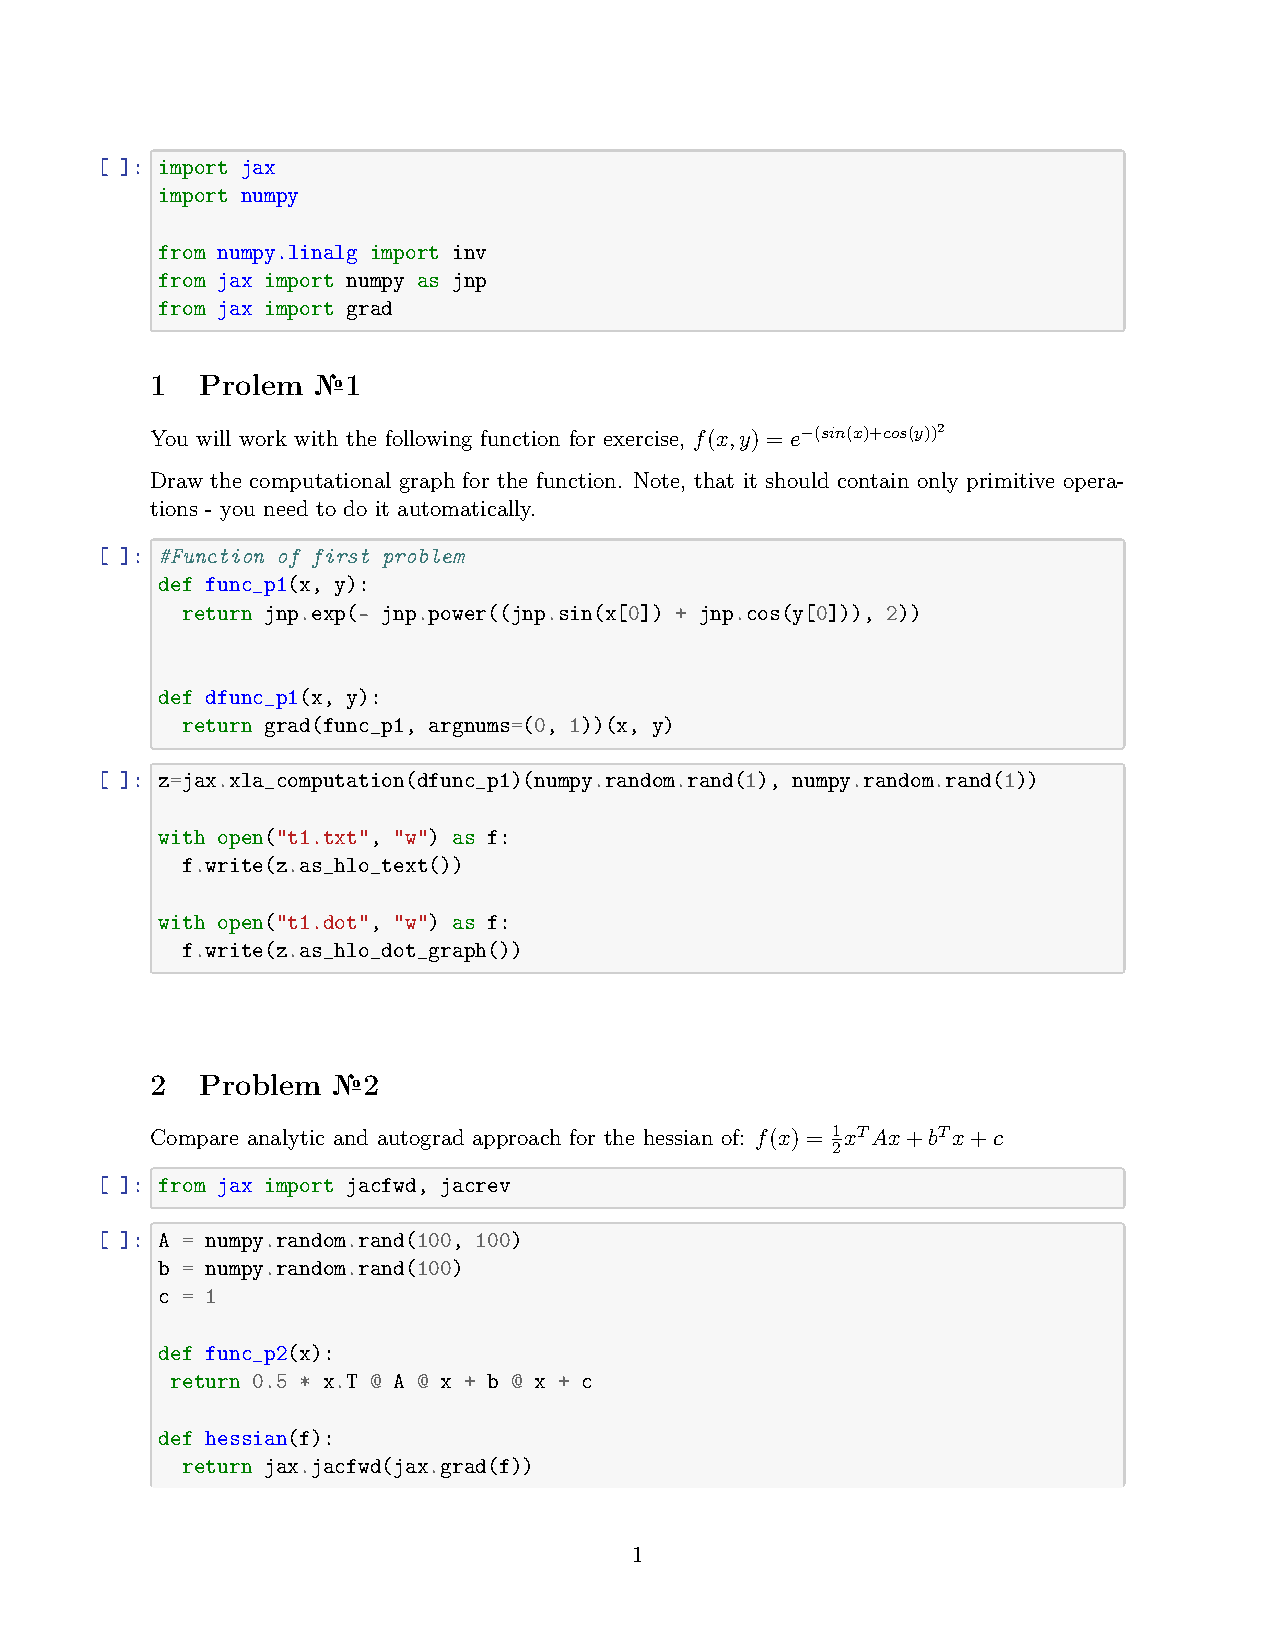
\includegraphics[width=0.991\textwidth, page=1]{task_03.pdf}    \newpage
 \includegraphics[width=\textwidth, page=2]{task_03.pdf}    
 \includegraphics[width=\textwidth, page=3]{task_03.pdf}    
 \newpage
 \includegraphics[width=\textwidth, page=4]{task_03.pdf}    
 \end{center}
 
  \section{Convex sets}

\subsection{Problem №1}

Show that the convex hull of the $\mathbf{S}$ set is the intersection of all convex sets containing $\mathbf{S}$

\underline{\textbf{Solution:}}

Firstly, we will prove that if A is a convex set, then any convex combination $x_1, .., x_n \in A$ will belong to A.

For $n = 1$ it's trivial.

Assume that this is true for any convex combination of n-1 points. Point $x = \sum\limits_{j=1}^n\alpha_j x_j$, $\sum\limits_{j=1}^n\alpha_j = 1$, $\alpha_1, ..., \alpha_n \in \mathds{R}$ and $n > 1$. Between $\alpha_1, ..., \alpha_n$ we can find $\alpha$ that will not be equal to 1. Without limiting the generality we consider that $\alpha \not = 1$.
\begin{equation*}
    \overline{\alpha_j} = \frac{\alpha_j}{1-\alpha_1}\text{, }j = 2, ..., n
\end{equation*}
Because $    \sum\limits_{j=2}^n\overline{\alpha_j} = 1 $
and from induction we can get that $ \overline{x} = \sum\limits_{j=1}^n\overline{\alpha_j}x_j \in A $
Then from convex of A we get:
\begin{equation*}
    x = \sum\limits_{j=1}^n\alpha_jx_j = \alpha_1x_1 + (1-\alpha_1)\sum\limits_{j=1}^n\frac{\alpha_j}{1-\alpha_1}x_j = \alpha_1 x_1 + (1-\alpha_1)\overline{x} \in A
\end{equation*}

From the proven it follows that if some convex set contains A, then it contains any convex combination of points from A, which means it contains convex hull of A. Let's show that convex hull of A is a convex set, in that case it coincides with the intersection of all convex sets containing A. Let's take random points from convex hull A. 
\begin{equation*}
    x = \sum\limits_{j=1}^n \alpha_jx_j \text{, } y = \sum\limits_{j = 1}^m \beta_jy_j
\end{equation*}
For any $\alpha \in [0, 1]$, we get:
\begin{equation*}
    (1-\alpha)x + \alpha y =\sum\limits_{j=1}^n(1-\alpha)\alpha_jx_j + \sum\limits_{j=1}^m\alpha \beta_j y_j
\end{equation*}

\begin{equation*}
    \sum\limits_{j=1}^n(1-\alpha)\alpha_j + \sum\limits_{j=1}^m\alpha \beta_j = (1-\alpha) + \alpha = 1
\end{equation*}
We get a convex combination of points $x_1, ..., x_n, y_1, ..., y_m$, which belongs to convex hull of A. 

WOHOO!!!


\subsection{Problem №2}
Show that the set of directions of the strict local descending of the differentiable function in a point is a convex cone.

\underline{\textbf{Solution:}}
It's trivial! Just imagine this picture in your mind, and it will become obvious, in general by definition.

\subsection{Problem №3}
Prove, that if S is convex, then $S + S = 2S$. Give a counterexample in case, when S -- is not convex.

\underline{\textbf{Solution:}} 
Let's show that: $2S \subseteq S + S:$ $\forall 2a \in 2S$, $\exists z= x + y \in S +S : z = 2a,$ $x, y \in S$. It's true, we can take $x = y = a$. We have proved that $2S \subseteq S +S$

Let's show that: $S + S \subseteq 2S:$ $\forall z \in S + S \exists 2a \in 2S : 2a = z$, $a = 0.5 x + 0.5 y$, $a \in S$ for reason that S is a convex set. And linear combination of its elements will belong to S. We prove that $S + S \subseteq 2S$.

It means that $S + S = 2S$.

\underline{\textbf{Counterexample:}} if S isn't convex. $S = \{0\} \bigcup [1, 2]$. 
\newline
$S + S = [0, 4]$, but $2S = {0} \bigcup [2, 4]$, $S + S \not = 2S$

\subsection{Problem №4}
Let $x \in \mathds{R}$ is a random variable with a given probability distribution of $\mathds{P}(x = a_i) = p_i$, where $i = 1, ..., n,$ and $a_1 < ... < a_n$. It is said the probability vector of outcomes of $p \in \mathds{R}^n$ belongs to the probabilistic simpex, i.e. $P = \{ p | \textbf{1}^Tp = 1, p \succcurlyeq 0\} = \{ p | p_1 + ... + p_n = 1, p_i \geq 0 \}$.
\newline
Determine if the following sets of p are convex:
\begin{itemize}
    \item $\alpha < \mathds{E} f(x) < \beta$, where $\mathds{E}f(x)$ stands for expected value of $f(x) : \mathds{R} \xrightarrow{} \mathds{R}$, i.e. $\mathds{E}f(x) = \sum\limits_{i=1}^n p_i\cdot f(a_i)$

    \item $\mathds{E}x^2 \leq \alpha$
    \item $\mathds{V}x \leq \alpha$
\end{itemize}

\underline{\textbf{Solution:}}

\underline{\textbf{A. }} It's right because we reduce constraints on p as constraints on the half-space, it will follow from this that the set is convex.

\begin{equation*}
    \alpha < \mathds{E} f(x) = \sum\limits_{i=1}^n p_if(a_i) < \beta
\end{equation*}
From the geometry it is half-space and convex, and it means that our set is also convex.


\underline{\textbf{B. }}
Here, we have the same idea like in \underline{\textbf{A.}}. We reduce constraints on p as constraints on the half-space, it will follow this that set is convex.
\begin{equation*}
\mathds{E} x^2 = \sum\limits_{i = 1}^n p_i a_i^2 \leq \alpha
\end{equation*}

\underline{\textbf{C.}}
\begin{equation*}
    0 \leq \mathds{V}x = \mathds{E}x^2 - (\mathds{E} x)^2 = \sum\limits_{i = 1}^n p_i a_i^2 - \left( \sum\limits_{i = 1}^n p_ia_i \right)^2 = -p^TXp + d^Tp \leq \alpha
\end{equation*}
where $d_i = a_i^2$ and $X = aa^T$, $X \succ 0$. This is a parabola with branches down in multidimensional space, it's concave function. And we also know that it will not be a convex set. For example, $-x^2 < 30$ will not be a convex set.

\underline{\textbf{Answer:}}
\textbf{A.-B.} convex. \textbf{C} is not convex.

\subsection{Problem №5}
Let $S \subset \mathds{R}^n$ is a set of solutions to the quadratic inequality:

\begin{equation*}
    S = \{x \in \mathds{R}^n \text{ | } x^TAx + b^Tx + c \leq 0 \}\text{; } A \in \mathds{S}^n, b \in \mathds{R}^n, c \in \mathds{R}
\end{equation*}
\begin{itemize}
    \item Show that if $A \succcurlyeq 0$, S is convex. Is the opposite true?
    \item Show that intersection of S with the hyperplane defined by the $g^Tx + h = 0$, $g \not = 0$ is convex if $A + \lambda gg^T \succcurlyeq 0$ for some $\lambda \in \mathds{R}$. Is the opposoite true?
\end{itemize}

\underline{\textbf{Solution:}}

\underline{\textbf{A.)}}
$x, y \in S$, $\theta \in [0, 1]$. If $\theta = 0$ or 1, it's trivial.

\begin{equation*}
    \theta x^TAx + \theta b^Tx + \theta c \leq 0
\end{equation*}

\begin{equation*}
    (1-\theta) y^TAy + (1-\theta) b^Ty + (1-\theta) c \leq 0
\end{equation*}

\begin{equation*}
    (\theta x + (1-\theta)y)^TA(\theta x + (1-\theta)y) + b^T(\theta x + (1-\theta)y) + c \leq 0
\end{equation*}

\begin{equation*}
    \theta^2 x^TAx + \theta(1-\theta)\left(y^TAx + x^TAy \right) + (1-\theta)^2 y^TAy + \theta b^Tx + (1-\theta)b^Ty + c \leq 0
\end{equation*}

Okay, lets' add $\theta x^TAx + (1-\theta)y^TAy$ and subtract it. 
\newline
$z = \theta^2 x^TAx + \theta(1-\theta)\left(y^TAx + x^TAy \right) + (1-\theta)^2 y^TAy - \theta x^TAx - (1-\theta)y^TAy $

\begin{equation*}
    z + \left(\theta x^TAx + \theta b^Tx + \theta c \right) + \left((1-\theta)y^TAy + (1-\theta)b^Ty + (1-\theta)c \right) \leq 0
\end{equation*}
From that
\begin{equation*}
    z = \theta^2 x^TAx + \theta(1-\theta)\left(y^TAx + x^TAy \right) + (1-\theta)^2 y^TAy - \theta x^TAx - (1-\theta)y^TAy  \leq 0
\end{equation*}

\begin{equation*}
    \theta(1-\theta) x^TAx + (1-\theta)\theta y^TAy \geq \theta(1-\theta)(y^Tax + x^TAy)
\end{equation*}

\begin{equation*}
    x^TA(x-y) + (y-x)^TAy \geq 0
\end{equation*}
It's right because $A \succcurlyeq 0$. 

\underline{\textbf{B.)}} I didn't do it.










 \section{Convex functions}

\subsection{Problem №1}
Is $f(x) = -x \cdot lnx - (1-x)ln(1-x)$ convex?

\underline{\textbf{Solution:}}

\begin{equation*}
    \nabla^2 f(x) = \frac{\partial}{\partial x} \left( -lnx - 1 + ln(1-x) + 1\right) = \frac{-1}{x} - \frac{-1}{1-x} = \frac{-1}{x(1-x)} < 0
\end{equation*}
because $x \in (0, 1)$ it is right. From this we get that f(x) is concave function, but not convex.

\underline{\textbf{Answer:}} No, it's not convex function, it's concave function.

\subsection{Problem №2}
Let x be a real variable with the values $a_1 < a_2 < ... < a_n$ with probabilities $\mathds{P} (x = a_i) = p_i$. Derive the convexity or concavity of the following functions from p on the set of $\left\{p \text{ | } \sum\limits_{i = 1}^n p_i = 1, \text{ } p_i \geq 0 \right)$

\underline{\textbf{Solution:}}
We know that linear function: $a^Tx + b$ convex and concave function at the same time.

\textbf{1.} $\mathds{E}x = \sum\limits_{i = 1}^n a_i \cdot p_i$ -- that's linear function, therefore math expectation is convex and concave function.

\textbf{2.} $\mathds{P} \{x \geq \alpha \} = \sum\limits_{i: a_i \geq \alpha} p_i$ -- it's linear function, therefore it's convex and concave function.

\textbf{3.} $\mathds{P} \{\alpha \leq x \leq \beta \} = \sum\limits_{i: \alpha \leq a_i \leq b_i}^n p_i$, we get that is convex and concave function.

\textbf{4.} $\sum\limits_{i = 1}^n p_i \log p_i$.

Okay, let's check is $f(x) = x \log x $ - convex

$\nabla^2f(x) = (x \log x)^{''} = (\log x + 1)^{'} = \frac{1}{x} > 0$, because $x > 0$ - yep, it's convex function. And our function is non-negative sum of convex function, then our function is convex function.

\textbf{5.} $\mathds{V} x = \mathds{E} (x-\mathds{E}x)^2 = \mathds{E}x^2 - \left( \mathds{E} x\right)^2$

Okay, let's take counterexample for this function:
\begin{enumerate}
    \item  $p_a = (1, 0)$, $x = (0, 1)$, $\mathds{V}x = 1 \cdot 1^2 - (1 \cdot 1)^2 = 0$

    \item $p_b = (0, 1)$, $x = (0, 1)$, $\mathds{V}x = 0 \cdot 1^2 + 1 \cdot 0^2 - (1 \cdot 0 + 0 \cdot 1)^2 = 0$

    \item $p_c = 0.5\cdot p_a + 0.5 \cdot p_b = (\frac{1}{2}, \frac{1}{2})$, $x = (0, 1)$,
    $\mathds{V}x = 0.5 \cdot 1^2 - (0.5 \cdot 1)^2 = 0.25$
\end{enumerate}

By definition of convex function the following equality is right:
\newline
\begin{equation*}
f(\theta x + (1-\theta)y ) \leq \theta f(x) + (1-\theta) f(y)    
\end{equation*}
But:
\begin{equation*}
    f(0.5p_a + 0.5p_b)=\frac{1}{4} \leq \frac{1}{2}f(p_a) + \frac{1}{2}f(p_b) = 0 + 0 = 0
\end{equation*}
And we get that it's not convex function, it's concave function.

\textbf{6.} \textbf{quatile}(x) = $\inf \{ \beta$ | $\mathds{P} \{x \leq \beta \} \geq 0.25\}$ 

$\inf$ is convex function, which is defined on probabilistic simplex, which is convex set, then \textbf{quartile}$(x)$ is convex function (Boyd 87 page, statement (3.16)).

\underline{\textbf{Answer:}}
\textbf{a-c} convex and concave function,  \textbf{d.} convex function, \textbf{e.} 
concave function. \textbf{f.} convex function.

\subsection{Problem №3}
Show, that $f(A) = \lambda_{max}(A)$ -- is convex, if $A \in S^n$

\underline{\textbf{Solution:}}
Okay, let's show that's is false if $A \in \mathds{R}^{2n}$:

Let's take: 
\begin{equation*}
    A = \begin{bmatrix}
    -8 & 16 \\
    60 & 4 
\end{bmatrix} \text{, }     B = \begin{bmatrix}
    2 & 40 \\
    20 & -2
\end{bmatrix}
\end{equation*}

\begin{equation*}
    \lambda_{max}(0.5 A + 0.5B) = \lambda_{max} \left( \begin{bmatrix}
        -3 & 28 \\
        40 & 1
    \end{bmatrix} \right) \leq 0.5 \lambda_{max}\left(\begin{bmatrix}
    -8 & 16 \\
    60 & 4 
\end{bmatrix} \right) + 0.5 \lambda_{max}\left( \begin{bmatrix}
    2 & 40 \\
    20 & -2
\end{bmatrix}\right)
\end{equation*}

$ \lambda_{max} \left( \begin{bmatrix}
        -3 & 28 \\
        40 & 1
    \end{bmatrix} \right)$, $\lambda_{max}\left( \begin{bmatrix}
        -3 & 28 \\
        40 & 1
    \end{bmatrix} \right) = 2(\sqrt{249} - 1)$, $\lambda_{max} \left(\begin{bmatrix}
    -8 & 16 \\
    60 & 4 
\end{bmatrix} \right) = 2\sqrt{201}$

\begin{equation*}
    \sqrt{1124} - 1 \approx 32.52 \leq \sqrt{249} - 1 + \sqrt{201} \approx 28.96
\end{equation*}

We see that the inequality for a convex function does not hold. Hence, it is not a convex function

\underline{\textbf{Solution:}}
If $A \in \mathds{S}^n$

We need to consider only diagonal matrix, because all others matrices we can get by multiplying by orthogonal matrices on both sides (they are the same because A - symmetric matrix, $A = \Sigma^T D \Sigma$).

And when we gonna find $\lambda(A) = det(A - \lambda I) = det(\Sigma^T D \Sigma - \lambda \Sigma^T \Sigma)  = \lambda(D - \lambda I)$, $D $-- diagonal matrix.

$\forall \theta \in (0, 1)$, for $\theta = 0$ or $\theta = 1$ it's trivial. $A, B$ -- diagonal matrices. 

\begin{equation*}
    \theta \cdot A + (1-\theta) \cdot B - \lambda I) = \begin{bmatrix}
    \theta \lambda_1^a + (1-\theta) \lambda_1^b  && 0 && ... \\
    0 & \theta \lambda_2^a + (1-\theta) \lambda_2^b && 0 \\
    \end{bmatrix}
\end{equation*}

And from that:
\begin{equation*}
    \lambda_{max}(\theta A + (1-\theta)B) = \sup\limits_{i = 1, n} ( \theta \lambda_i^a + (1-\theta) \lambda_i^b) \leq \theta \cdot \sup\limits_{i = 1, n}(\lambda_{i}^a) + (1-\theta)\sup\limits_{i = 1, n}(\lambda_i^b)
\end{equation*}

\begin{equation*}
    \theta \cdot \sup\limits_{i = 1, n}(\lambda_{i}^a) + (1-\theta)\sup\limits_{i = 1, n}(\lambda_i^b) = \theta \lambda_{max}(A) + (1-\theta)\lambda_{max}(B)
\end{equation*}

Wohoo, we proved that $\lambda_{max}$ is convex function.

\underline{\textbf{Alternative solution:}}
$\lambda_{max}(A) = \max\limits_{||u|| = 1} \langle u, Au \rangle$. 

We know that $f(A) = \langle u, Au \rangle$ is linear function, which means it's convex function. $max$ is convex non-decreasing function. And from that we get that composition of this function is convex function.

Wohoo, we proved that $\lambda_{max}$ is convex function.

\subsection{Problem №4}
Prove that, $f(X) = - \log \det X$ is convex on $X \in \mathds{S}_{++}^n$

\underline{\textbf{Solution:}}
\begin{equation*}
df(x) = - \frac{1}{detX} detX \langle X^{-T}, dX \rangle = - \langle X^{-T}, dX \rangle
\end{equation*}

\begin{equation*}
    d^2f(x) = -d(tr(X^{-1}, dX_1) = -tr(d(X^{-1})dX_1) = tr(X^{-1}dX_2X^{-1}dX_1)
\end{equation*}
For a reason that $X^{-1}, dX_1, dX_2 \in \mathds{S}_{++}^n$ trace is positive, the hessian of f(x) is positive, then we get that f(x) is convex function on $\mathds{S}_{++}^n$. 
In later I understand that $dX_1$ and $dX_2$ can be non positive matrices. And this is an unfair statement.

\underline{\textbf{Alternative solution:}}
Let's take: $X = A + tB$, $A \in \mathds{S}_{++}^n, B \in \mathds{S}^n$, $t$ is such for which $A + tB \succ 0$. We can represent A as $A = CC$, $det(A) = det(CC) = (detC)^2$.
\newline 
$F(t) = \log det(A + tB)$.

\begin{equation*}
    F(t) = \log det(A + tB) = \log det(CC + tB) = \log det(C(I + t C^{-1}BC^{-1})C) 
\end{equation*}

\begin{equation*}
    F(t) = \log det(I + tC^{-1}BC^{-1}) + \log detA
\end{equation*}
Let's write $C^{-1}BC^{-1} = U \Sigma V^*$, $\Sigma = diag(\lambda_1, ..., \lambda_n)$, because it's symmetric, $U = V$, then:
\begin{equation*}
    F(t) = \log det(UU^* + tU\Sigma U^*) + \log detA = \log det(U(I + t\Sigma)U^*) + \log detA 
\end{equation*}

\begin{equation*}
    F(t) = \log det(I + t \Sigma) + \log detA = \log \prod\limits_{i=1}^n(1 + t \lambda_i) + \log detA= \sum\limits_{i=1}^n \log(1 + t\lambda_i) + \log detA
\end{equation*}
Then F(t) is concave function, because it's sum of concave functions. Then we get that $-F(t)$ is convex function. Wohoo, we proved it.


\subsection{Problem №5}

Prove, that adding $\lambda ||x||_2^2$ to any convex function $g(x)$ ensures strong convexity function of a resulting function $f(x) = g(x) + \lambda ||x||_2^2$. Find the constant of the strong convexity $\mu$.

\underline{\textbf{Solution:}}
\begin{equation*}
    \frac{\partial^2}{\partial x_l \partial x_k} \sum\limits_{i = 1}^n x_i = \frac{\partial}{\partial x_l} 2x_k = 0
\end{equation*}
\begin{equation*}
    \frac{\partial^2}{(\partial x_k)} \sum\limits_{i = 1}^n x_i = \frac{\partial}{\partial x_k} 2x_k = 2
\end{equation*}
The hessian of $||X||_2^2$ is $2 I$. Then $\nabla^2 f(x) = \nabla^2 g(x) + \lambda \cdot 2I \succcurlyeq \lambda I$. It's right because g(x) is convex function.

\subsection{Problem №6}
Study the following function of two variables $f(x, y) = e^{xy}$.
\begin{enumerate}
    \item[a.] Is this function convex?
    \item[b.] Prove, that this function will be convex on the line $x=y$.
    \item[c.] Find another set in $\mathds{R}^2, on which this function will be convex$
\end{enumerate}

\underline{\textbf{Solution:}}
\begin{enumerate}
    \item[a.] No this function is not convex on $\mathds{R}^2$, because the hessian equals $-(1+2xy)e^{2xy}$ and it is less than zero for $x = 0, y = 1$.
    \item[b.] $f(x, x) = e^{x^2}$, $\nabla^2 f(x) = 2(1+2x^2)e^{x^2} > 0$, $\forall x \in \mathds{R}$, and from that we get that $f(x)$ is strong convex function.
    \item[c.] Let's take $y = x^3$, $f(x, x) = e^{x^4}$, $\nabla^2 f(x) = (12x^2 + 16x^6)e^{x^4} \geq 0 $, $\forall x \in \mathds{R}$
\end{enumerate}

\underline{\textbf{Answer:}} 
\textbf{a.} No, this function is not convex on $\mathds{R}^2$, \textbf{b.} proved, \textbf{c.} $y = x^3$

\subsection{Problem №7}
Show, that the following function is convex on  the set of all positive denominators:
\begin{equation*}
    f(x) \frac{1}{x_1 - \frac{1}{x_2 - \frac{1}{x_3 - \frac{1}{...}}}}, \text{ , } x \in \mathds{R}^n
\end{equation*}

\underline{\textbf{Solution:}}
$f_n = \frac{1}{x_n}, f_{n-1} = \frac{1}{x_{n-1} - f_n}$
\newline 
Let's make induction from n to n-1: $(f_n)^{''} = \frac{2}{x_n^3} > 0$, $x_n > 0$.
\newline 
$n - 1$: $f_{n-1} = \frac{1}{x_{n-1} - f_n}$, 
\begin{equation*}
    \nabla^2 f_{n-1}(x) = 
    \begin{bmatrix}
    \frac{2}{(x_{n-1}-f_n)^3} & \frac{2}{x_n^2(x_{n-1} -f_n)^3} \\
    \frac{2}{x_n^2(x_{n-1} -f_n)^3} & \frac{2}{x_n^3(x_n-f_n)^2} + \frac{2}{x_n^4(x_{n-1} - f_n)^3} 
    \end{bmatrix}
\end{equation*}
\begin{enumerate}
    \item $\frac{2}{(x_{n-1}-f_n)^3} > 0$ it's true by a condition of a task.

    \item $|\nabla^2f(x)| = \frac{4}{x_n^3(x_{n-1}-f_n)^3} + \frac{4}{x_n^4(x_{n-1}-f_n)^6} - \frac{4}{x_n^4(x_{n-1}-f_n)^6} = \frac{4}{x_n^3(x_{n-1} -f_n)^3} > 0$
\end{enumerate}

Wohoo, $\nabla^2 f_{n-1}(x)$ is positive defined matrix, it's means that $f_{n-1}$ is convex function.

By induction we get that $f_1(x)$ is convex function.

\underline{\textbf{Alternative solution:}}
Exists a statement: if $\phi(x)$ is convex function that is monotonously decreasing and $\alpha(x)$ is concave function, than $f(x) = \phi(\alpha(x))$ will be convex function. 
For our example: $\phi(x) = 1/x)$, $\phi(x)$ -- convex function, and $\alpha_k(x) = x_k - \phi(a_{k+1})$ is concave function, $\phi(x) = \alpha_n(x) = 1/x$, $-\alpha_i(x)$ is concave function.
\newline
We can represent f in the form of:
$f(x) = \phi(x_1 - \phi(x_2 - \phi(x_{3} - ... \phi(x_{n-1} - \phi(x_n))...)$ will be convex function based on this statement. (3.2.4 Scalar composition, 84 page Optimization Boyd)

 \section{Conjugate sets}
%\subsection{Problem №1}
%Find the sets $\mathds{S}^*, \mathds{S}^{**}, \mathds{S}^{***}$, if

%\begin{equation*}
%    \mathds{S} = \{ x \in \mathds{R}^2 \text{ | } x_1 + x_2 \geq -1, \text{ } 2x_1 - x_2 \geq 0, \text{ } -x_1+2x_2\leq -2\}
%\end{equation*}

%\underline{\textbf{Solution:}}

%\underline{\textbf{Answer:}}

\subsection{Problem №4}
Find the conjugate set to the ellipsoid:
\begin{equation*}
    S = \left\{ x \in \mathds{R}^n | \sum\limits_{i=1}^n a_i^2x_i^2 \leq \varepsilon^2 \right\}
\end{equation*}

\underline{\textbf{Solution:}}
It's equivalent to:
\begin{equation*}
    S = \left\{ x \in \mathds{R}^n | \sum\limits_{i=1}^n a_i^2x_i^2 \leq \varepsilon^2 \right\}
\end{equation*}
$A = diag(\frac{a_i}{\varepsilon})$
\begin{equation*}
    ||Ax||_2^2 = \sum\limits_{i=1}^n (\frac{a_i}{\varepsilon})^2x_i^2
\end{equation*}

From Boyd's optimization I know that:
\begin{equation*}
S = \{ x \in \mathds{R}^n | ||Ax||_2 \leq 1 \} = E = \{ A^{-1}u | ||u||_2 \leq 1\}    
\end{equation*}
$A^{-1} = diag(\frac{\epsilon}{a_i})$. 

Let's show that it's true.
\newline
1. $E \subseteq S$: $x = A^{-1}u$, $||u||_2 \leq 1$ в S: $||AA^{-1}u||_2 \leq 1$, therefore $E \subseteq S$ it's true.
\newline
2. $S \subseteq E$: $||Ax||_2 \leq 1$, $z = Ax$, $||z||_2 \leq 1$, $x = A^{-1}z$, $||z||_2 \leq 1$, therefore $x\ \in E$, $\hookrightarrow S \subseteq E$

We prove that it's true. 

We need find all $p \in E^* : \forall x \in E$, $\langle p, x \rangle \geq -1$, $\forall x = A^{-1}u$, $||u||_2 \leq 1$, 
\begin{equation*}
\langle p, A^{-1}u \rangle = \langle A^{-T}p, u \rangle \geq -1    
\end{equation*}

From cauchy-bunyakovsky and $||u||_2 \leq 1$ we get:
\begin{equation*}
    |\langle A^{-T}p, u \rangle|\leq ||u||_2 \cdot ||A^{-T}p||_2 \leq ||A^{-T}p||_2 
\end{equation*}

We are suitable for all p, for which is true: $\langle A^{-T}p, u \rangle = - ||A^{-T}p||_2$,
$-||A^{-T}p||_2 \geq -1$, we get:
\begin{equation*}
    ||A^{-T}p||_2 \leq 1
\end{equation*}
This sets an ellips with matrix $A^{-T} = diag(\frac{\varepsilon}{a_i})$.

\begin{equation*}
    S^* = E^* = \left\{ x \in \mathds{R}^n | \sum\limits_{i=1}^n (\frac{\varepsilon}{a_i})^2 x_i^2 \leq 1 \right\}
\end{equation*}

\underline{\textbf{Answer:}}

\begin{equation*}
    S^* = \left\{ x \in \mathds{R}^n | \sum\limits_{i=1}^n (\frac{1}{a_i})^2 x_i^2 \leq \frac{1}{\varepsilon^2} \right\}
\end{equation*}
 \section{Conjugate functions}

\subsection{Problem №1} Find $f^*(y)$, if $f(x) = p \cdot x - q$

\underline{\textbf{Solution:}}

\begin{equation*}
    f^*(y) = \sup_{x \in dom(f)} \left( 
    \langle y, x \rangle - f(x) \right) = \sup_{x \in \mathbf{R}} \left( xy - px + q\right)
\end{equation*}

$g(x) = xy - px + q$, $\nabla g(x) = y - p$
And we can easy get a answer:

\underline{\textbf{Answer:}} $f^*(y) = \begin{cases}
   q, y = p \\
   +\inf , y \ne p.
 \end{cases}$

\subsection{Problem №2}
Find $f^*(y), if f(x) = \frac{1}{2}x^TAx$, $A \in \mathbf{S}_{++}^n$

\underline{\textbf{Solution:}}

\begin{equation*}
    f^*(y) = \sup_{x \in dom(f)} \left( 
    \langle y, x \rangle - f(x) \right) = \sup_{x \in \mathbf{R}^n} \left( y^Tx - \frac{1}{2}x^TAx\right)
\end{equation*}

$g(x) = y^Tx - \frac{1}{2}x^TAx$

$\nabla g(x) = y - Ax$, because $A \in \mathbf{S}_{++}^n$, $\nabla g(x) = 0 \hookrightarrow$
$y = Ax$

\begin{equation*}
    f^*(y) = \sup_{x \in \mathbf{R}^n}\left( (Ax)^Tx - \frac{1}{2}x^TAX\right) = \sup_{x \in \mathbf{R}^n}\left( \frac{1}{2}x^TAX\right) = + \infty
\end{equation*}

\underline{\textbf{Answer:}} $f^*(y) = +\infty$

\subsection{Problem №3}
Find $f^*(y), if f(x) = log \left( \sum\limits_{i=1}^n e^{x_i}\right)$

\underline{\textbf{Solution:}}

\begin{equation*}
    f^*(y) = \sup_{x \in dom(f)} \left( 
    \langle y, x \rangle - f(x) \right) = \sup_{x \in \mathbf{R}^n} \left( y^Tx - log \left( \sum\limits_{i=1}^n e^{x_i}\right)
    \right)
\end{equation*}

$d(y^tx - f(x)) = \langle y, dx \rangle - \frac{\langle e^x, dx \rangle}{\sum\limits_{i=1}^n e^{x_i}}=0$,  $e^x$ in meaning that it equals $(e^{x_1}, e^{x_2}, ..., e^{x_n})$.

And we get that: $y = \frac{e^x}{\sum\limits_{i=1}^n e^{x_i}}$

\begin{equation*}
    f^*(y) = \sup_{x \in \mathbf{R}^n} \left(\sum\limits_{i=1}^n y_ix_i - log \left( \sum\limits_{i=1}^n e^{x_i}\right) \right) = \sup_{x \in \mathbf{R}^n} \left(\sum\limits_{i=1}^n log(e^{y_ix_i}) - log \left( \sum\limits_{i=1}^n e^{x_i}\right) \right) 
\end{equation*}

\begin{equation*}
    f^*(y) = \sum\limits_{i=1}^n log \left( \frac{e^{y_i}e^{x_i}}{\sum\limits_{k=1}^n e^{x_k}} \right) = \sum\limits_{i=1}^n log \left( e^{y_i}y_i \right) = \sum\limits_{i=1}^n y_i log(y_i) 
\end{equation*}

Oh wow, it's crossentropyloss ( $y \succ 0$, $y^T\mathds{1} = 1$, so y - probability vector)

Now we need to find dom $f^*$. 
\begin{enumerate}
    \item if $\exists y_i$ : $y_i < 0$, let's take $x_j = -\alpha$, and $x_l$ for all l : $l \not = j$, then:
    \begin{equation*}
    y^tx - f(x) = \alpha - log \alpha \xrightarrow{\alpha \xrightarrow{} +\infty} +\infty    
    \end{equation*}

    \item if $y \succ 0$, but $y^T \mathds{1} \not = 1$, let's take $x = \alpha \cdot \mathds{1}$
    \begin{equation*}
    y^Tx - f(x) = y^T\alpha\mathds{1} - \alpha  - \log(n)
    \end{equation*}
    
    if $y^T \mathds{1} > 1$, then we take $\alpha \xrightarrow{} +\infty$ and get that $f^*(y) = +\infty$

    if $y^T\mathds{1} < 1$, then we take $\alpha \xrightarrow{} -\infty$ and get that $f^*(y) = -\infty$
\end{enumerate}

\underline{\textbf{Answer:}}
\begin{equation*}
f^*(y) = \begin{cases}
    \sum\limits_{i = 1}^n y_i \cdot log(y_i), \text{if } \succ 0 \text{ and } y^T\mathds{1} = 1 \\
    +\infty, otherwise
\end{cases}    
\end{equation*}

\subsection{Problem №4}
Prove, that if $f(x) = g(Ax),$ then $f^*(y) = g^*(A^{-T}y)$

\underline{\textbf{Solution:}}
\begin{equation*}
f^*(y) = \sup_{x \in \mathbf{R}^n}\left(y^Tx - f(x)  \right)
\end{equation*}

$y^Tdx - \nabla f(x)^Tdx = 0$, $y = \nabla f(x)$
\begin{equation*}
    f^*(y) \sup_{x \in \mathbf{R}^n} \left( (\nabla f(x))^Tx - f(x) \right)
\end{equation*}

The same way we can get:
%\[ \adjustlimits\\sup_{a\in A} \inf_{b\in B} \mathrm{d}(a,b) \]

\begin{equation*}
    g^*(y) = \sup_{x \in \mathbf{R}^n} \left( (\nabla g(x))^Tx - g(x) \right)
\end{equation*}

\begin{equation*}
    g^*(A^{-T}y) = \sup_{x \in \mathbf{R}^n} \left( (A^{-T}\nabla(g(x))^Tx - g(x) \right)
\end{equation*}

$x = Ax_1$

\begin{equation*}
    g^*(A^{-T}y) = \sup_{x_1 \in \mathbf{R}^n} \left( \nabla g(Ax_1)^T A^{-1}Ax_1 - g(Ax_1) \right) = \sup_{x_1 \in \mathbf{R}^n} \left( \nabla g(Ax_1)^Tx_1 - g(Ax_1)
    \right)
\end{equation*}

Because $g(Ax_1) = f(x_1)$, we can get:

\begin{equation*}
    g^*(A^{-T}y) = \sup_{x_1 \in \mathbf{R}^n} \left( \nabla f(x_1)^Tx_1 - f(x_1)\right) = f^*(y)
\end{equation*}
    
WOHOO!

\subsection{Problem №5}
Find $f^*(Y)$, if $f(X) = -\log( det X), X \in \mathbf{S}_{++}^n$

\underline{\textbf{Solution:}}

\begin{equation*}
    f^*(Y) = \sup_{x \in \mathbf{R}^{n \times n}} \left( \langle Y, X \rangle + \log(detX) \right)
\end{equation*}

$\langle Y, dX \rangle + \frac{1}{detX}d(detX) = \langle Y, dX \rangle + \frac{1}{detX}detX \langle X^{-T}, dX \rangle = 0$

And we get: $Y = - X^{-T}$, $X = -Y^{-T}$

\begin{equation*}
    f^*(Y) = \langle Y, - Y^{-T} \rangle + \log(det(-Y^{-1})) = tr(-E) + \log \left(det(-Y^{-1}) \right)
\end{equation*}

\begin{equation*}
    f^*(Y) = -n + \log \left(det(-Y^{-1}) \right)
\end{equation*}

\underline{\textbf{Answer:}}

\begin{equation*}
    f^*(Y) = -n + log(det(-Y^-1)), \text{ where } Y \in -\mathds{S}_{++}^n
\end{equation*}
 \section{Subgradient and subdifferential}


\subsection{Problem № 1} 
Find $\partial f(x)$, if $f(x) = $ \textbf{Leaky ReLU}$(x) = $ $\begin{cases}
   x, if x > 0 \\
   0.01x , otherwise
 \end{cases}$
 
\underline{\textbf{Solution:}}
By Dubovitsky-Milutin theorem we can get:
\begin{equation*}
    \partial f(x) = \begin{cases}
        1, x > 0 \\
        [0.01; 1], x = 0 \\
        0.01, x < 0 
    \end{cases}
\end{equation*}

\underline{\textbf{Answer:}}
$
    \partial f(x) = \begin{cases}
        1, x > 0 \\
        [0.01; 1], x = 0 \\
        0.01, x < 0 
    \end{cases}
$
\subsection{Problem №2}
Find subdifferential of a function $f(x) = cosx$ on the set $X = [0, \frac{3}{2} \pi ]$.

\underline{\textbf{Solution:}}
\begin{center}
    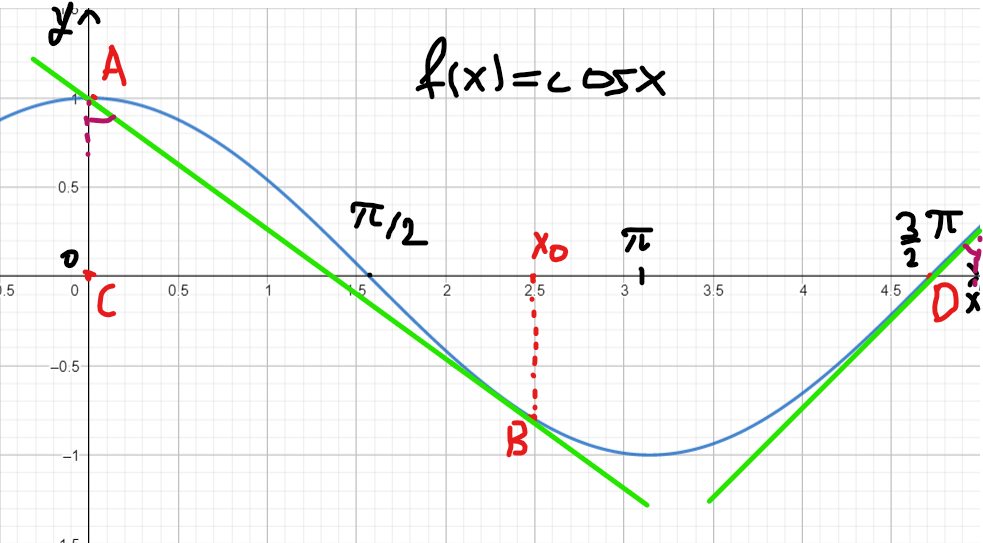
\includegraphics[scale=0.7]{pictures/task_07_01.png}
\end{center}

\underline{\textbf{Answer:}}
$
    \partial f(x) = \begin{cases}
        [-\infty, -sinx], x = 0 \\
        \varnothing, x \in (0, x_0) \\
        -sinx, x \in [x_0, \frac{3}{2} \pi) \\
        [1, +\infty], x = \frac{3}{2} \pi
    \end{cases}
$

\subsection{Problem №3}
Find $\partial f(x)$, if $f(x) = ||Ax - b||_1^2$

\underline{\textbf{Solution:}}
By property of subdifferential we can get 
that:
\begin{equation*}
\partial(||Ax - b||_1^2) = ||Ax - b||_1 \partial(||Ax-b||_1)     
\end{equation*}
From the seminar we know that:
\begin{equation*}
    \partial||y||_1 = \{\alpha : ||\alpha||_{\infty} \leq 1, \alpha^Ty = ||y||_1\}
\end{equation*}
And now we can get that (by another property of subdifferential:
\begin{equation*}
    \partial\left(||Ax - b||_1^2 \right) = ||Ax - b||_1 \partial \left(||Ax-b||_1 \right)(x) = ||Ax - b||_1A^T \partial ||Ax+b||_1
\end{equation*}


\begin{equation*}
 ||Ax - b||_1A^T \partial ||Ax+b||_1 = ||Ax - b||_1A^T \cdot \{\alpha : ||\alpha||_{\infty} \leq 1, \alpha^T (Ax+b ) = ||Ax+b||_1\}
\end{equation*}

\underline{\textbf{Answer:}} $\partial f(x) = ||Ax - b||_1A^T \cdot \{\alpha : ||\alpha||_{\infty} \leq 1$, $\alpha^T (Ax+b ) = ||Ax+b||_1\}$

\subsection{Problem №4}
Suppose, that if $f(x) = ||x||_{\infty}$. Prove that $\partial f(0) = $ \textbf{conv} $\{\pm e_1, ..., \pm e_n \}$, where $e_i$ is i-th canonical basis vector (column of identity matrix).

\underline{\textbf{Solution:}}
By the definition: $f(x) = ||x||_{\infty} = \max\limits_i |x_i|$

We know that subbdifferential for module is equal:
\begin{equation*}
    \partial |x_i| = \begin{cases} 
    x_i, x_i > 0\\
    [-1, 1], x_i = 0 \\
    -x_i, x_i < 0
    \end{cases}
\end{equation*}

Because $|x_i|$ -- convex functions, by Dubovitsky - Milutin theorem we can get:
\begin{equation*}
    \partial f(0) = conv \left\{ \bigcup\limits_{i \in \overline{1, n}} \partial|x_i|_{x_i = 0} \right\} = conv \left\{\pm e_1, ..., \pm e_n\right\}\text{, } e_i \text{ is i-th canonical basis vector}
\end{equation*}

WOHOO, we proved that!

\subsection{Problem №5}
Find $\partial f(x)$, if $f(x) = e^{||x||}$. \\Try do the task for an arbitrary norm. At least, try $||\cdot || = ||\cdot||_{\{2, 1, \infty \}}$

\underline{\textbf{Solution:}}
\newline
By the property of subdifferential we: $\partial f(x) = \partial(e^{||x||}) = e^{||x||} \partial(||x||)$
\newline
And now we need to find $\partial ||x||$ for $||x||_1, ||x||_2$ and $||x||_{\infty}$
\newline
\textbf{1.}
In the seminar we find that and it equals: 
\begin{equation*}
\partial||x||_1 = \{\alpha : ||\alpha||_{\infty} \leq 1, \alpha^Tx = ||x||_1\}
\end{equation*}
\newline
\textbf{2.}
By definition $||x||_2 = \sqrt{\sum\limits_{i = 1}^n x_i^2}$, this function is differentiable everywhere except zero. 
\newline
For $x \not = 0$, $\partial f(x) = \nabla ||x||_2 =\frac{x}{||x||_2}$
\newline
Now we need to consider $x = 0$: let's find such interesting limit: $\lim\limits_{\beta \xrightarrow{} 0+} \frac{||\beta e||_2}{\beta} = ||e||_2$, where e is unit vector on unit sphere.

But by definition $\frac{x}{||x||_2} = e$,  and we get that 
\begin{equation*}
\partial ||x||_2 = \{e \text{ | } ||e||_2 \leq 1 \}    
\end{equation*}
\newline
\textbf{3.}
In \underline{problem №4} I find that ($x_i$ - maximum element by modules):
\begin{equation*}
    ||x||_{\infty} = \begin{cases}
            [-1, 1], \text{ if } i x_i = 0 \\
            sign(x_i), x_i \not = 0
    \end{cases}
\end{equation*}

\underline{\textbf{Answer:}}

\begin{itemize}
    \item for $|| \cdot ||_1$: $\partial f(x) = e^{||x||_1} \cdot \{\alpha : ||\alpha||_{\infty} \leq 1, \alpha^Tx = ||x||_1\}$
    \item for $|| \cdot ||_2$: $\partial f(x) = e^{||x||_2} \cdot \{e \text{ | } ||e||_2 \leq 1 \}$
    \item for $|| \cdot ||_{\infty}$: $\partial f(x) = e^{||x||_{\infty}} \cdot \begin{cases}
            [-1, 1], \text{ if } x_i = 0 \\
            sign(x_i), x_i \not = 0
    \end{cases}$, where is $x_i$ -- maximum element by modules
\end{itemize}



 \section{Conjugate functions}

\subsection{Problem № 1} Find $f^*(y)$, if $f(x) = p \cdot x - q$

\underline{\textbf{Solution:}}

\begin{equation*}
    f^*(y) = \sup_{x \in dom(f)} \left( 
    \langle y, x \rangle - f(x) \right) = \sup_{x \in \mathbf{R}} \left( xy - px + q\right)
\end{equation*}

$g(x) = xy - px + q$, $\nabla g(x) = y - p$
And we can easy get a answer:

\underline{\textbf{Answer:}} $f^*(y) = \begin{cases}
   q, y = p \\
   +\inf , y \ne p.
 \end{cases}$

\subsection{Problem №2}
Find $f^*(y), if f(x) = \frac{1}{2}x^TAx$, $A \in \mathbf{S}_{++}^n$
\underline{\textbf{Solution:}}

\begin{equation*}
    f^*(y) = \sup_{x \in dom(f)} \left( 
    \langle y, x \rangle - f(x) \right) = \sup_{x \in \mathbf{R}^n} \left( y^Tx - \frac{1}{2}x^TAx\right)
\end{equation*}

$g(x) = y^Tx - \frac{1}{2}x^TAx$

$\nabla g(x) = y^T - xA )$, because $A \in \mathbf{S}_{++}^n$
$y = A^Tx$

\begin{equation*}
    f^*(y) = \sup_{x \in \mathbf{R}^n}\left( (A^Tx)^Tx - \frac{1}{2}x^TAX\right) = \sup_{x \in \mathbf{R}^n}\left( \frac{1}{2}x^TAX\right) = +\inf
\end{equation*}

\underline{\textbf{Answer:}} $f^*(y) = +inf$

\subsection{Problem №3}
Find $f^*(y), if f(x) = log \left( \sum\limits_{i=1}^n e^{x_i}\right)$

\underline{\textbf{Solution:}}

\begin{equation*}
    f^*(y) = \sup_{x \in dom(f)} \left( 
    \langle y, x \rangle - f(x) \right) = \sup_{x \in \mathbf{R}^n} \left( y^Tx - log \left( \sum\limits_{i=1}^n e^{x_i}\right)
    \right)
\end{equation*}

$d(y^tx - f(x)) = \langle y, dx \rangle - \frac{\langle e^x, dx \rangle}{\sum\limits_{i=1}^n e^{x_i}}=0$,  $e^x$ in meaning that it equals $(e^{x_1}, e^{x_2}, ..., e^{x_n})$.

And we get that: $y = \frac{e^x}{\sum\limits_{i=1}^n e^{x_i}}$

\begin{equation*}
    f^*(y) = \sup_{x \in \mathbf{R}^n} \left(\sum\limits_{i=1}^n y_ix_i - log \left( \sum\limits_{i=1}^n e^{x_i}\right) \right) = \sup_{x \in \mathbf{R}^n} \left(\sum\limits_{i=1}^n log(e^{y_ix_i}) - log \left( \sum\limits_{i=1}^n e^{x_i}\right) \right) 
\end{equation*}

\begin{equation*}
    f^*(y) = \sum\limits_{i=1}^n log \left( \frac{e^{y_i}e^{x_i}}{\sum\limits_{k=1}^n e^{x_k}} \right) = \sum\limits_{i=1}^n log \left( e^{y_i}y_i \right) = \sum\limits_{i=1}^n y_i log(y_i) 
\end{equation*}

Oh wow, it's crossentropyloss ( $y \succ 0$, $y^T\mathbf{1} = 1$, so y - probability vector)


\underline{\textbf{Answer:}}

\subsection{Problem №4}
Prove, that if $f(x) = g(Ax),$ then $f^*(y) = g^*(A^{-T}y)$

\underline{\textbf{Solution:}}
\begin{equation*}
f^*(y) = \sup_{x \in \mathbf{R}^n}\left(y^Tx - f(x)  \right)
\end{equation*}

$y^Tdx - \nabla f(x)^Tdx = 0$, $y = \nabla f(x)$
\begin{equation*}
    f^*(y) \sup_{x \in \mathbf{R}^n} \left( (\nabla f(x))^Tx - f(x) \right)
\end{equation*}

The same way we can get:
%\[ \adjustlimits\\sup_{a\in A} \inf_{b\in B} \mathrm{d}(a,b) \]

\begin{equation*}
    g^*(y) = \sup_{x \in \mathbf{R}^n} \left( (\nabla g(x))^Tx - g(x) \right)
\end{equation*}

\begin{equation*}
    g^*(A^{-T}y) = \sup_{x \in \mathbf{R}^n} \left( (A^{-T}\nabla(g(x))^Tx - g(x) \right)
\end{equation*}

$x = Ax_1$

\begin{equation*}
    g^*(A^{-T}y) = \sup_{x_1 \in \mathbf{R}^n} \left( \nabla g(Ax_1)^T A^{-1}Ax_1 - g(Ax_1) \right) = \sup_{x_1 \in \mathbf{R}^n} \left( \nabla g(Ax_1)^Tx_1 - g(Ax_1)
    \right)
\end{equation*}

Because $g(Ax_1) = f(x_1)$, we can get:

\begin{equation*}
    g^*(A^{-T}y) = \sup_{x_1 \in \mathbf{R}^n} \left( \nabla f(x_1)^Tx_1 - f(x_1)\right) = f^*(y)
\end{equation*}
    
WOHOO!

\subsection{Problem №5}
Find $f^*(Y)$, if $f(X) = -\log( det X), X \in \mathbf{S}_{++}^n$

\underline{\textbf{Solution:}}

\begin{equation*}
    f^*(Y) = \sup_{x \in \mathbf{R}^{n \times n}} \left( \langle Y, X \rangle + \log(detX) \right)
\end{equation*}

$\langle Y, dX \rangle + \frac{1}{detX}d(detX) = \langle Y, dX \rangle + \frac{1}{detX}detX \langle X^{-T}, dX \rangle = 0$

And we get: $Y = - X^{-T}$, $X = -Y^{-T}$

\begin{equation*}
    f^*(Y) = \langle Y, - Y^{-T} \rangle + \log(det(-Y^{-1})) = tr(-E) + \log \left((-1)^n det(Y^{-1}) \right)
\end{equation*}

\begin{equation*}
    f^*(Y) = -n + \log \left( \frac{(-1)^n}{detY} \right)
\end{equation*}

\underline{\textbf{Answer:}}
$f^*(Y) = \log \left( \frac{(-1)^n}{detY} \right) - n$
 \section{Duality}

\subsection{Problem №1}
Express the dual problem of
\begin{equation*}
    c^Tx \rightarrow 1\min_{x \in \mathds{R}^n}
\end{equation*}
\begin{equation*}
    \text{s.t. } f(x) \leq 0
\end{equation*}
with $c \not = 0$, in terms of the conjugate function $f^*$. Explain why the problem you give is convex. We do not assume f is convex.

\underline{\textbf{Solution:}}
Let's write lagrangian ($\lambda \geq 0, \lambda \in \mathds{R}^n$):
\begin{equation*}
    L(x, \lambda) = c^Tx + \lambda f(x) 
\end{equation*}
\begin{equation*}
    g(\lambda) = \inf_{x \in \mathds{R}^n}(c^Tx + \lambda f(x)) = - \lambda \sup_{x \in \mathds{R}^n} (-\frac{1}{\lambda}c^Tx - f(x)) = \text{ } | \text{ by definition } | \text{ } = - \lambda f^*(-\frac{c}{\lambda}) 
\end{equation*}

Okay, let's write dual problem.

\begin{equation*}
    -\lambda f^*(-\frac{c}{\lambda}) \rightarrow \max_{\lambda \in \mathds{R}}
\end{equation*}
\begin{equation*}
    \text{s. t. } \lambda \geq 0
\end{equation*}

\underline{\textbf{Answer:}} It's concave function

\subsection{Problem №2}
Minimum volume covering ellipsoid. Let we have the primal problem:
\begin{equation*}
    \log \det X^{-1} \rightarrow \min_{X \in \mathds{S}_{++}^n}
\end{equation*}
\begin{equation*}
    \text{s. t. } a_i^TXa_i \leq 1 \text{, } i = 1, ..., m
\end{equation*}
\begin{enumerate}
    \item Find Lagrangian of the primal problem
    \item Find the dual function
    \item Write down the dual problem
    \item Check whether problem holds strong duality or not
    \item Write down the solution of the dual problem
\end{enumerate}

\underline{\textbf{Solution:}}
$f_i(X) = a_i^TXa_i - 1$, $f(X) = (f_1, ..., f_m)$.
\begin{enumerate}
\item
\begin{equation*}
    L(x, \lambda) = \log \det X^{-1} + \sum\limits_{i=1}^m \lambda_i (a_i^TXa_i - 1)= \log \det X^{-1} + \lambda^T f(X)
\end{equation*}

\item  We can really easy find the dual function for this problem, because we have already find the conjugate function in first homework.
\begin{equation*}
    f^*(Y) = -n + \log \det(-Y^{-1}) \text{, where } Y \in \mathds{S}_{++}^n
\end{equation*}

\begin{equation*}
    g(\lambda, \nu) = -b^T\lambda - d^T\nu - f_0^*(-A^T\lambda-C^T\nu)
\end{equation*}

\begin{equation*}
    g(\lambda) = \begin{cases}
     \log \det \left( \sum\limits_{i=1}^m \lambda_i a_ia_i^T \right) 
      - \mathds{1}^T \lambda + n, \sum\limits_{i=1}^m \lambda_i a_ia_i^T \succ 0 \\
      
     +\infty \text{, otherwise}
    \end{cases}
\end{equation*}


\item

\begin{equation*}
    \log \det \left(\sum\limits_{i=1}^m(\lambda_i a_ia_i^T) \right) + n - \lambda^T\mathds{1} \rightarrow \max_{\lambda \in \mathds{R}^m}
\end{equation*}
\begin{equation*}
    \text{s. t. } \lambda \succcurlyeq 0
\end{equation*}

\item Strong duality holds, because Slater's conditions are performed, it menas that $\exists X \in \mathds{S}_{++}^n$ such that $a_i^TXa_i < 1$, $i \in \overline{1, m}$

\item Let's solve it! From fully symmetric problem and many iterations, when I am trying to solve this problem, I get that $\lambda $ will be like that $\lambda = (\alpha, \alpha, ..., \alpha)$.

Okay, it's feasible to our budget set, let's put in our function.

\begin{equation*}
    g(\lambda) = \log \det \left(\sum\limits_{i=1}^m(\alpha a_ia_i^T) \right) + n - \alpha m = 
    \log \alpha^n \det \left(\sum\limits_{i=1}^m a_ia_i^T \right) + n - \alpha m
\end{equation*}

Okay, from it we need to maximize only: $h(\alpha) = n \log \alpha - \alpha m$, it's concave function and local maximum will be global.

\begin{equation*}
    h'(\alpha) = \frac{n}{\alpha} - m = 0
\end{equation*}
From it we get that: $\alpha^* = \frac{n}{m}$ and $h(\alpha^*) = n \log \frac{n}{m} - n$
\begin{equation*}
    g(\lambda^*) = \log \det \left(\sum\limits_{i=1}^m a_ia_i^T \right) + n \log \frac{n}{m}
\end{equation*}

We all remember, that:
\begin{equation*}
    \nabla_X L(X, \lambda) = -X^{-1} + \sum\limits_{i=1}^m \lambda_i a_ia_i^T = 0
\end{equation*}

\begin{equation*}
    \nabla_{\lambda} L(X, \lambda) = \sum\limits_{i=1} (a_i^TXa_i - 1) = 0
\end{equation*}
Okay, let's show that $\nabla_{\lambda} L(X^*, \lambda^*) = 0$, if $X^-1 = \sum\limits_{i=1}^m \lambda_i a_ia_i^T$.

\begin{equation*}
    \nabla_{\lambda} L \sum\limits_{i=1}(a_i^T \left( \sum\limits_{i=1}^m \alpha a_ia_i^T \right)^{-1} a_i) - m = 
    \sum_{i=1}^m \langle a_ia_i^T, \left( \sum\limits_{i=1}^m \alpha a_ia_i^T \right)^{-1} \rangle - m 
\end{equation*}

And we get:
\begin{equation*}
    \langle \sum_{i=1}^m  a_ia_i^T,  \left( \sum\limits_{i=1}^m \alpha a_ia_i^T \right)^{-1} \rangle - m = \frac{n}{\alpha} - m = \text{ } | \text{ } \alpha = \frac{n}{m} | \text{ } = \frac{n}{n/m} - m = 0
\end{equation*}
Youhoo, our $\alpha^*$ is feasible for Slater's conditions. And if we input $X^*$ into $f_0(X)$ we will get:

\begin{equation*}
    f_0(X^*) = \log \det (\sum\limits_{i=1}^m \alpha a_ia_i^T) = n \log \alpha + \log \det \sum\limits_{i=1}^m a_ia_i^T  = n \log \frac{n}{m} + \log \det \sum\limits_{i=1}^m a_ia_i^T
\end{equation*}
\begin{equation*}
    g(\lambda^*) =  \log \det \sum\limits_{i=1}^m a_ia_i^T  + n \log \frac{n}{m}
\end{equation*}
We show strong duality and solve duality problem.

\end{enumerate}

\subsection{Problem №3}
A penalty method for equality constraints. We consider the problem of minimization.

\begin{equation*}
f_0(x) \rightarrow \min_{x \in \mathds{R}^n}
\end{equation*}
\begin{equation*}
    \text{s. t. } Ax = b
\end{equation*}
where $f_0(x) : \mathds{R}^n \xrightarrow{} \mathds{R}$ is convex and differentiable, and $A \in \mathds{R}^{m \dot n}$ with rank$A = m$.

In a quadratic penalty method, we form an auxiliary function:
\begin{equation*}
    \phi (x) = f_0(x) + \alpha ||Ax - b||_2^2
\end{equation*}
where $\alpha > 0$ is a parameter. This auxiliary function consists of the objective plus the penalty term $\alpha ||Ax - b||_2^2$. The idea is that a minimizer of the auxiliary function, $\widetilde{x}$, should be an approximate solution of the original problem. Intuition suggests that the larger the penalty weight $\alpha$, the better the approximation $\widetilde{x}$ to a solution of the original problem. Suppose $\widetilde{x}$ is a minimizer of $\phi(x)$. Show how to find, from $\widetilde{x}$, a dual feasible point for the original problem. Find the corresponding lower bound on the optimal value of the original problem.

\underline{\textbf{Solution:}}
Let's write lagrangian:
\begin{equation*}
    L(x, \lambda) = f_0(x) + \lambda^T(Ax -b )
\end{equation*}

\begin{equation*}
\nabla_x L(x, \lambda) = \nabla f_0(x) + A^T \lambda    
\end{equation*}

If $\widetilde{x}$ is min in $\phi(x)$, then we get:
\begin{equation*}
    \nabla \phi(\widetilde{x}) = \nabla f_0(\widetilde{x}) + 2\alpha A^T(A\widetilde{x} - b) = 0
\end{equation*}
And from that we get:
\begin{equation*}
    \lambda  = 2 \alpha(A\widetilde{x} -b)
\end{equation*}

Let's write the dual problem to that:

\begin{equation*}
    g(\lambda) = \inf_{x \in \mathds{R}^n} (f_0(x) + \lambda^T(Ax - b) = f_0(\widetilde{x}) + 2\alpha ||A\widetilde{x} - b|_2^2
\end{equation*}
And for all x such that: $Ax = b$
\begin{equation*}
    f_0(x) \geq f_0(\widetilde{x}) + 2\alpha ||A\widetilde{x} - b||_2^2
\end{equation*}

And when we increasing alpha we get higher lower bound for the original problem.

\subsection{Problem №4}
Analytic centering. Derive a dual problem for

\begin{equation*}
- \sum\limits_{i=1}^m \log (b_i - a_i^Tx) \rightarrow \min_{x \in \mathds{R}^n}
\end{equation*}

\begin{equation*}
    \text{with domain } \{x | a_i^T x < b_i, i \in \overline{1, m} \}
\end{equation*}

First introduce new variables $y_i$ and equality constraints $y_i = b_i - a_i^Tx$. (The solution of this problem is called the analytic center of the linear inequalities $a_i^Tx \leq b_i$, $i \in \overline{1, m}$. Analytic centers have geometric applications, and play an important role in berrier methods).

\underline{\textbf{Solution:}}
Let's take $y_i = b - a_i^Tx$.
\begin{equation*}
    L(x, y, \nu) = - \log \sum\limits_{i=1}^m \log y_i + \sum\limits_{i=1}^m\nu_i(y_i - b_i + a_i^Tx)
\end{equation*}

The dual function will be:
\begin{equation*}
    g(\nu) = \inf_{x, y \in domain} ( - \sum\limits_{i=1}^m \log y_i + \sum\limits_{i=1}^m\nu_i(y_i + a_i^Tx)) + \nu^Tb
\end{equation*}

If $\sum\limits_{i=1}^m \nu_i a_i^T = \nu^TA = 0$ it's not true, than it will unbounded bellow. If $\nu \not \succ 0$ it will be also unbounded below. Let's write our function, the optimal is $y_i = \frac{1}{\nu_i}$.

\begin{equation*}
    g (\nu) = \begin{cases}
        \sum\limits_{i=1}^m \log \nu_i + m - \nu^Tb \text{, } \nu^TA = 0\text{, } \nu \succ 0 \\
        -\infty \text{, otherwise}
    \end{cases}
\end{equation*}

Dual problem will be:
\begin{equation*}
 \sum\limits_{i=1}^m \log \nu_i + m -\nu^T b \rightarrow \max_{\nu \in \mathds{R}^m}
\end{equation*}

\begin{equation*}
    \text{s.t. } \nu^TA = 0
\end{equation*}
 \section{Linear Programming}

\subsection{Problem №1}
The company’s production facilities are such that if we devote the entire production to headphones covers, we can produce 5000 of them in one day. If we devote the entire production to phone covers or laptop covers, we can produce 4000 or 2000 of them in one day.

The production schedule is one week (6 working days), and the week’s production must be stored before distribution. Storing 1000 headphones covers (packaging included) takes up 30 cubic feet of space. Storing 1000 phone covers (packaging included) takes up 50 cubic feet of space, and storing 1000 laptop covers (packaging included) takes up 220 cubic feet of space. The total storage space available is 1500 cubic feet.

Due to commercial agreements with Random Corp has to deliver at least 4500 headphones covers and 3000 laptop covers per week in order to strengthen the product’s diffusion.

The marketing department estimates that the weekly demand for headphones covers, phone, and laptop covers does not exceed 9000 and 14000, and 7000 units, therefore the company does not want to produce more than these amounts for headphones, phone, and laptop covers.

Finally, the net profit per each headphones cover, phone cover, and laptop cover is 5, 7 and 12 \$, respectively.

The aim is to determine a weekly production schedule that maximizes the total net profit.

\begin{enumerate}
    \item[a.]  Write a Linear Programming formulation for the problem. Use following variables:
    $y_1, y_2, y_3$ - number of covers for headpnones, phones and laptops produced per week.
    \item[b.] Finf the solution to the problem using PyOMO.
\end{enumerate}

\underline{\textbf{Solution:}}


\begin{equation*}
    \begin{bmatrix} 5, 7, 12 \end{bmatrix} 
    \begin{bmatrix}
    y_1 \\
    y_2 \\
    y_3
    \end{bmatrix}  \rightarrow \max_{y \in \mathds{R}^3}
\end{equation*}

\begin{equation*}
    \begin{gathered}
        s.t. \left(y_1 \frac{30}{1000} + y_2 \frac{50}{1000} + y_3 \frac{220}{1000} \right) \leq 1500 \\
        4500 \leq y_1 \leq 9000 \\
        0 \leq y_2 \leq 14000 \\
        3000 \leq y_3 \leq 7000 \\
        \frac{y_1}{5000} + \frac{y_2}{4000} + \frac{y_3}{2000} \leq 6
    \end{gathered}
\end{equation*}

Let's rewrite this problem in terms of x: $y_1 = x_1 + 4500$, $y_2 = x_2$, $y_3 = x_3 + 3000$.

\begin{equation*}
    \begin{bmatrix} 5, 7, 12 \end{bmatrix} 
    \begin{bmatrix}
    x_1 \\
    x_2 \\
    x_3
    \end{bmatrix} + 58500 \rightarrow \max_{x \in \mathds{R}^3}
\end{equation*}


\begin{equation*}
    \begin{gathered}
        s.t. \left(x_1 \frac{30}{1000} + x_2 \frac{50}{1000} + x_3 \frac{220}{1000} \right) \leq 705 \\
        0 \leq x_1 \leq 4500 \\
        0 \leq x_2 \leq 14000 \\
        0 \leq x_3 \leq 4000 \\
        \frac{x_1}{5000} + \frac{x_2}{4000} + \frac{x_3}{2000} \leq 3.6
    \end{gathered}
\end{equation*}


\begin{center}
    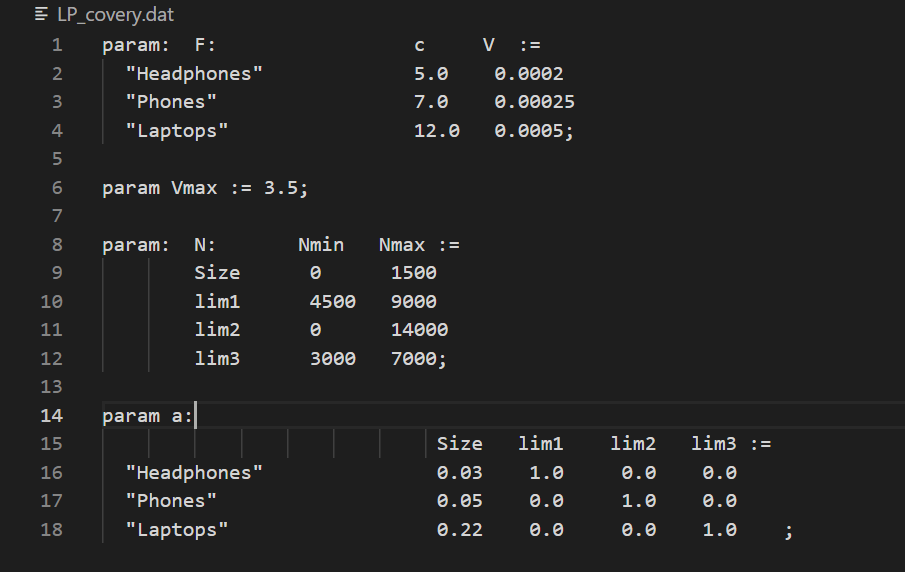
\includegraphics[scale=0.6]{pictures/task_11_ydat.png} \\
    data for linear programming in terms of y
\end{center}

\begin{center}
    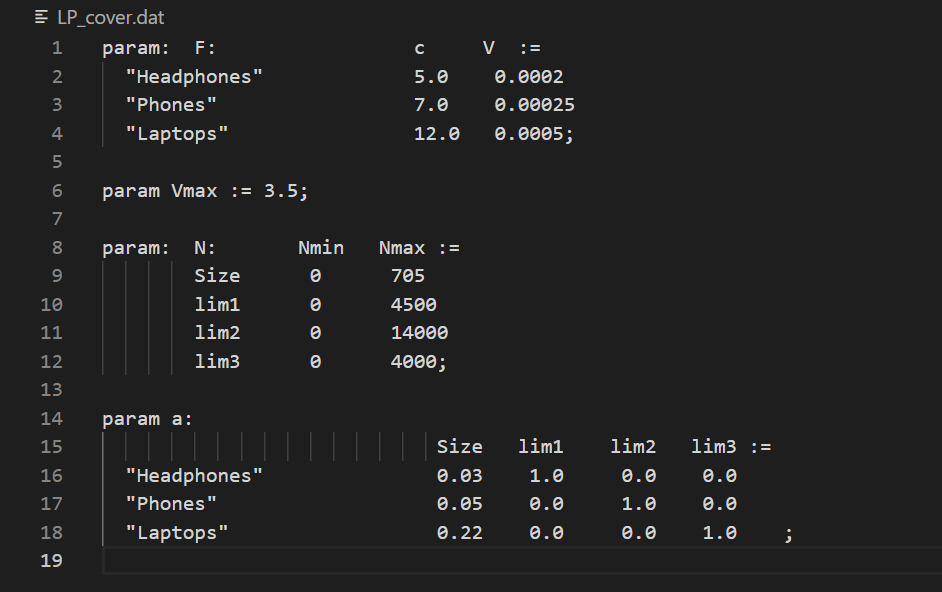
\includegraphics[scale=0.6]{pictures/task_11_xdat.png} \\
    data for linear programming in terms of x
\end{center}

\begin{center}
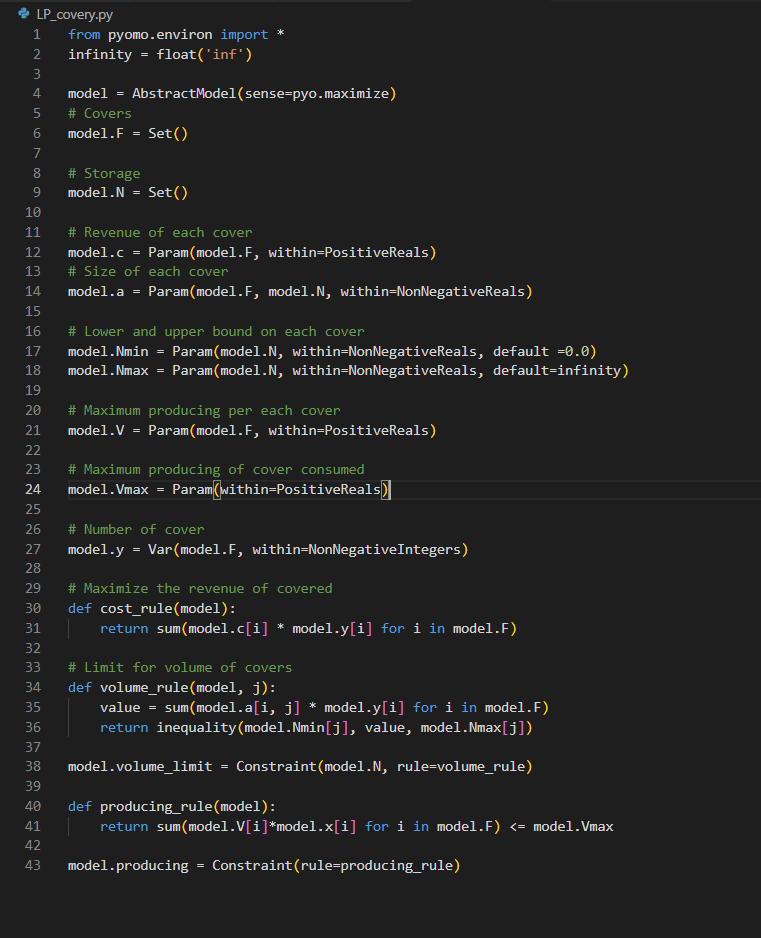
\includegraphics[scale=0.9]{pictures/task_11_ypy.png} \\
solutions in terms of y
\end{center}

\begin{center}
    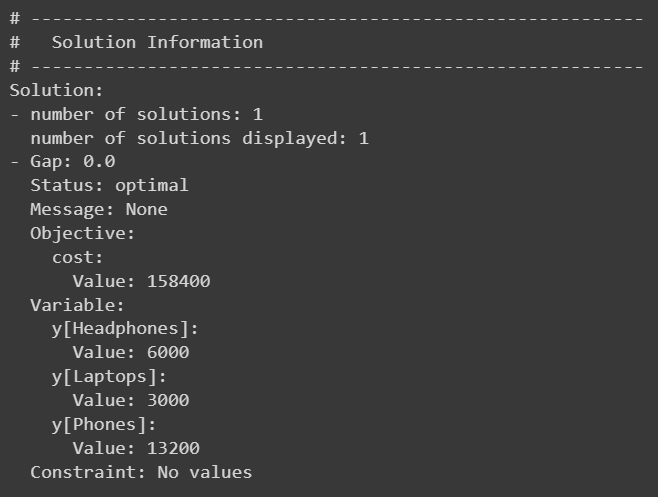
\includegraphics[scale=0.58]{pictures/task_11_yans.png} \\
    answer problem in terms of y
\end{center}

\begin{center}
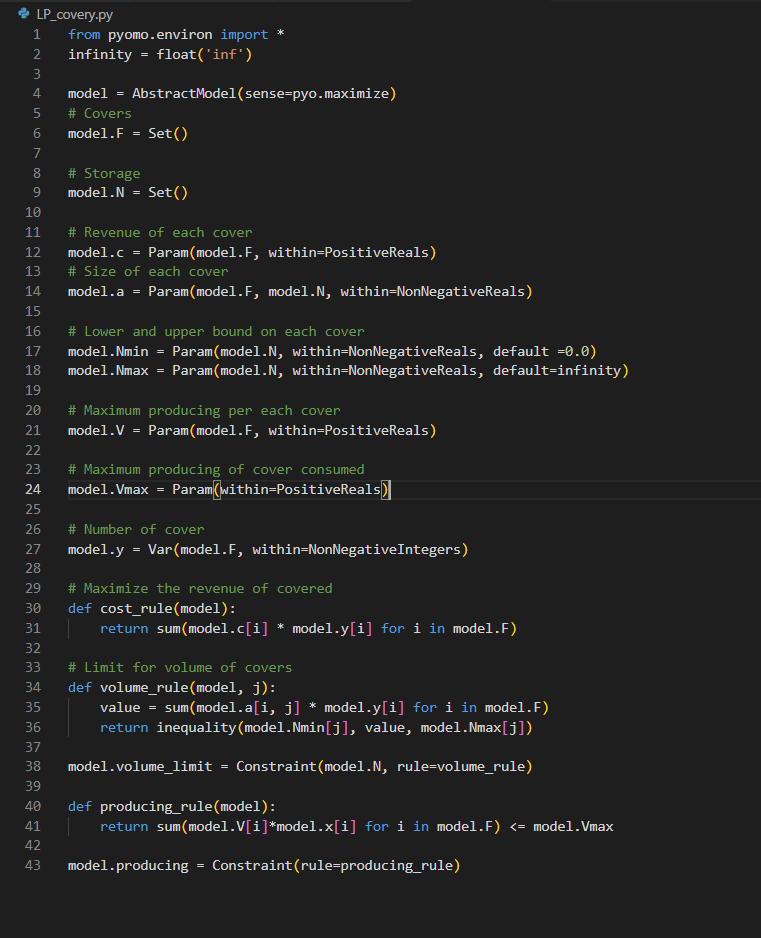
\includegraphics[scale=0.9]{pictures/task_11_xpy.png} \\
solutions in terms of x
\end{center}

\begin{center}
    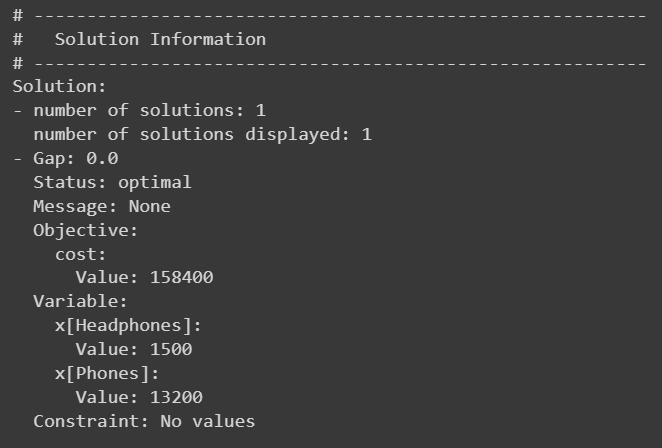
\includegraphics[scale=0.58]{pictures/task_11_xans.png} \\
    answer problem in terms of x
\end{center}


\subsection{Problem №2}
Prove the optimality of the solution
\begin{equation*}
    x^T = \left( \frac{5}{26}, \frac{5}{2}, \frac{27}{26} \right)
\end{equation*}

to the following linear programming problem:
\begin{equation*}
    9x_1 + 14x_2 + 7x_3 \rightarrow \max_{x \in \mathds{R}^n}
\end{equation*}

\begin{equation*}
\begin{gathered}
    \text{s.t. } 2x_1 + x_2 + 3x_3 \leq 6 \\
    5x_1 + 4x_2 + x_3 \leq 12 \\
    2x_2 \leq 5
\end{gathered}
\end{equation*}
buy you cannot use any numerical algorithm here.

\underline{\textbf{Solution:}}
Point $x = \left( 0, 0, 0 \right)^T$ satisfies Slater's conditions.

\begin{equation*}
\begin{gathered}
        0 < 6  \\
        0 < 12 \\
        0 < 5
\end{gathered}
\end{equation*}
And KKT becomes necessary and sufficient.

\begin{equation*}
    L(x, \lambda) = 9x_1 + 14x_2 + 7x_3 - \lambda_1(2x_1 + x_2 + 3x_3 - 6) - \lambda_2(5x_1 + 4x_2 + x_3 - 12) - \lambda_3 (2x_2 -5)
\end{equation*}

\begin{equation*}
    \begin{cases}
    \nabla_{x_1} L = 9  - 2\lambda_1 - 5\lambda_2 = 0 \\
    \nabla_{x_2} L = 14 - \lambda_1  - 4\lambda_2 - 2\lambda_3 = 0 \\
    \nabla_{x_3} L = 7  - 3\lambda_1 - \lambda_2 = 0 \\
    \lambda \succcurlyeq 0 \\
    \lambda_1 (2x_1 + x_2 + 3x_3 - 6) = 0 \\
    \lambda_2 (5x_1 + 4x_2 + x_3 - 12) = 0 \\
    \lambda_3 (2x_2 - 5) = 0 \\
    2x_1 + x_2 + 3x_3 \leq 6 \\
    5x_1 + 4x_2 + x_3 \leq 12 \\
    2x_2 \leq 5
    \end{cases}
\end{equation*}
From it we get:
\begin{equation*}
\begin{cases}
    \lambda_1 = 2 \\
    \lambda_2 = 1 \\
    \lambda_3 = 4 \\
    \lambda \succcurlyeq 0 \\
    2\cdot(2 \cdot \frac{5}{26} + \frac{5}{2} + 3 \cdot \frac{27}{27} - 6) = 2\cdot(6 -6) = 0 \\
    1 \cdot(5 \cdot \frac{5}{26} + 4 \cdot \frac{5}{2} + \frac{27}{27} - 12) = 12 - 12 = 0 \\
    4 \cdot (2 \frac{5}{2} - 5) = 0 \\
    2 \cdot \frac{5}{26} + \frac{5}{2} + 3 \cdot \frac{27}{27} = 6 \leq 6 \\  
    5 \cdot \frac{5}{26} + 4 \cdot \frac{5}{2} + \frac{27}{27} = 12 \leq 12 \\
    2 \frac{5}{2} = 5 \leq 5
\end{cases}
\end{equation*}
\begin{equation*}
    L(\frac{5}{26}, \frac{5}{2}, \frac{27}{26}) = 9 \cdot \frac{5}{26} + 14 \frac{5}{2} + 7 \frac{27}{26} - 2 \cdot(6-6) - (12 - 12) - 4 \cdot (5 - 5) = \frac{45 + 70 + 189}{26} = \frac{304}{26}
\end{equation*}
Optimal point: $\frac{152}{13}$

We show that this problem satisfies Slater's conditions and KKT becomes essential and suffiecient condition. And point $x = \left( \frac{5}{26}, \frac{5}{2}, \frac{27}{26} \right)^T$ satisfies the conditions of the KKT.

\subsection{Problem №3}
Transform the following linear program into an equivalent linear programm in standart form($c^Tx \rightarrow \max_{x \in \mathds{R}^n} : Ax = b, x \geq 0$):


\begin{equation*}
    x_1 - x_2 \rightarrow \min_{x \in \mathds{R}^n}
\end{equation*}

\begin{equation*}
\begin{gathered}
    \text{s.t. } 2x_1 + x_2 \geq 3 \\
    3x_1 - x_2 \leq 7 \\
    x_1 \geq 0
\end{gathered}
\end{equation*}

\underline{\textbf{Solution:}}

Let's take $x_1 = x$, $X_2 = y - z$, where $y = x_{2+}$, $z = x_{2-}$, $y, z \geq 0$
And rewrite our problem.

\begin{equation*}
    x_1 - x_2 \rightarrow \min_{x \in \mathds{R}^3}
\end{equation*}

\begin{equation*}
\begin{gathered}
    \text{s.t. } -2x_1 - y + z \leq 3 \\
    3x_1 - y + z \leq 7 \\
    x_1 \geq 0 \\
    y \geq 0 \\
    z \geq 0
\end{gathered}
\end{equation*}
Okay, let's again rewrite it.

\begin{equation*}
    x - y + z \rightarrow \min_{x \in \mathds{R}^3}
\end{equation*}

\begin{equation*}
\begin{gathered}
    \text{s.t. } 
    \begin{pmatrix}
    2  & 1  & -1 \\
    3  & -1 & 1 \\
    -1 & 0  & 0 \\
    0  & -1 & 0 \\
    0  & 0  & -1 
    \end{pmatrix} 
    \begin{bmatrix}
    x \\
    y \\
    z
    \end{bmatrix} \succcurlyeq \begin{pmatrix}
        3 \\
        3 \\
        0 \\
        0 \\
        0
    \end{pmatrix} 
\end{gathered}
\end{equation*}
But we need to rewrite it standart form, not it's canonical form.

\begin{equation*}
\begin{gathered}
    c = \left(1, -1, 0\right)^T \\
    A = \begin{pmatrix}
    2  & 1  & -1 \\
    3  & -1 & 1 \\
    -1 & 0  & 0 \\
    0  & -1 & 0 \\
    0  & 0  & -1 
    \end{pmatrix} \\
    b = \left(3, 3, 0, 0, 0\right)^T
\end{gathered}
\end{equation*}

\begin{equation*}
    L(x, \lambda) = c^Tx + \lambda^T(Ax - b) = (c^T + \lambda^TA-)x - \lambda^T b
\end{equation*}
\begin{equation*}
    g(\lambda) = \inf_{x \in \mathds{R}^3} \left(c^T + \lambda^TA \right)x - \lambda^T b
\end{equation*}

And we have: 
\begin{equation*}
    -b^T\lambda\rightarrow \max_{\lambda \in \mathds{R}^5}
\end{equation*}

\begin{equation*}
\begin{gathered}
    \text{s.t. } A^T\lambda = - c \\
    \lambda \succcurlyeq 0
\end{gathered}
\end{equation*}

And finally:
\begin{equation*}
    -\left(3, 3, 0, 0, 0 \right)^T\lambda\rightarrow \max_{\lambda \in \mathds{R}^5}
\end{equation*}
\begin{equation*}
\begin{gathered}
    \text{s.t. } \begin{pmatrix}
    2  & 3  & -1 & 0  & 0  \\
    1  & -1 & 0  & -1 & 0  \\
    -1 & 1  & 0  & 0  & -1 \\
    \end{pmatrix} \lambda = (-1, 1, 0)^T \\
    \lambda \succcurlyeq 0
\end{gathered}
\end{equation*}

\subsection{Problem №4}
Consider
\begin{equation*}
    4x_1 + 5x_2 + 2x_3 \rightarrow \max_{x \in \mathds{R}^3}
\end{equation*}
\begin{equation*}
\begin{gathered}
    \text{s.t. } 2x_1 - x_2 + 2x_3 \leq 9 \\
    3x_1 + 5x_2 + 4x_3 \leq 8 \\
    x_1 + x_2 + 2x_3 \leq 2 \\
    x_1, x_2, x_3 \geq 0
\end{gathered}
\end{equation*}
\begin{enumerate}
    \item[a] Find an optimal solution to the Linear Programming using the simplex method.
    \item[b] Write the dual linear program. Find an optimal dual solution. Do we have strong duality here?
\end{enumerate}

\underline{\textbf{Solution:}}
Let's rewrite problem to normal canonical form (by scheme from lecture): 
\begin{equation*}
    \begin{gathered}
        4x_1 + 5x_2 + 2x_3 - x_7 - x_8 - x_9  \rightarrow \max_{x \in \mathds{R}^9}\\
        \text{s.t.  } 2x_1 - x_2 + 2x_3 + x_4 + x_7 = 9\\
                     3x_1 + 5x_2 + 4x_3 + 4x_4 + x_5 + x_8 = 8 \\
                     x_1 + x_2 + x_3 + x_6 + x_9 = 2 \\
                     x_1, x_2, x_3, x_4, x_5, x_6, x_7, x_8, x_9 \geq 0 
    \end{gathered}
\end{equation*}
$4x_1 + 5x_2 + 5x$

First table of simplex method:
\begin{table}[H]
\begin{tabular}{|l|l|l|l|l|l|l|l|l|l|l|l|l|}
\hline
      & c* &    & 0  & 0  & 0  & 0  & 0  & 0  & -1 & -1 & -1 &     \\ \hline
Basis &    & b   & a1 & a2 & a3 & a4 & a5 & a6 & a7 & a8 & a9 & t   \\ \hline
a7    & -1 & 9   & 2  & -1 & 2  & 1  & 0  & 0  & 1  & 0  & 0  & 4.5 \\ \hline
a8    & -1 & 8   & 3  & 5  & 4  & 0  & 1  & 0  & 0  & 1  & 0  & 2   \\ \hline
a9    & -1 & 2   & 1  & 1  & 2  & 0  & 0  & 1  & 0  & 0  & 1  & 1   \\ \hline
z     &    & -19 & -6 & -5 & -8 & -1 & -1 & -1 & -1 & -1 & -1 &     \\ \hline
delta &    &     & -6 & -5 & -8 & -1 & -1 & -1 & 0  & 0  & 0  &     \\ \hline
\end{tabular}
\end{table}

New basis: $a_3, a_7, a_8$.

\begin{table}[H]
\begin{tabular}{|l|l|l|l|l|l|l|l|l|l|l|l|l|}
\hline
      & c* &     & 0   & 0   & 0  & 0  & 0  & 0   & -1 & -1 & -1  &   \\ \hline
Basis &    & b   & a1  & a2  & a3 & a4 & a5 & a6  & a7 & a8 & a9  & t \\ \hline
a3    & 0  & 1   & 0.5 & 0.5 & 1  & 0  & 0  & 0.5 & 0  & 0  & 0.5 & 2 \\ \hline
a7    & -1 & 7   & 1   & -2  & 0  & 1  & 0  & -1  & 1  & 0  & -1  & 7 \\ \hline
a8    & -1 & 4   & 1   & 3   & 0  & 0  & 1  & 2   & 0  & 1  & 2   & 4 \\ \hline
z     &    & -11 & -2  & -1  & 0  & -1 & -1 & -1  & -1 & -1 & -1  &   \\ \hline
delta &    &     & -2  & -1  & 0  & -1 & -1 & -1  & 0  & 0  & 0   &   \\ \hline
\end{tabular}
\end{table}

New basis: $a_1, a_7, a_8$

\begin{table}[H]
\begin{tabular}{|l|l|l|l|l|l|l|l|l|l|l|l|l|}
\hline
      & c* &    & 0  & 0  & 0  & 0  & 0  & 0  & -1 & -1 & -1 &     \\ \hline
Basis &    & b  & a1 & a2 & a3 & a4 & a5 & a6 & a7 & a8 & a9 & t   \\ \hline
a1    & 0  & 2  & 1  & 1  & 2  & 0  & 0  & 1  & 0  & 0  & 1  & --- \\ \hline
a7    & -1 & 5  & 0  & -3 & -2 & 1  & 0  & -2 & 1  & 0  & -2 & 5   \\ \hline
a8    & -1 & 2  & 0  & 2  & 2  & 0  & 1  & -3 & 0  & 1  & -3 & --- \\ \hline
z     &    & -7 & 0  & 1  & 0  & -1 & -1 & 5  & -1 & -1 & 5  &     \\ \hline
delta &    &    & 0  & 1  & 0  & -1 & -1 & 5  & 0  & 0  & 6  &     \\ \hline
\end{tabular}
\end{table}

New basis: $a_1, a_7, a_5$.
\begin{table}[H]
\begin{tabular}{|l|l|l|l|l|l|l|l|l|l|l|l|l|}
\hline
      & c* &    & 0  & 0  & 0  & 0  & 0  & 0  & -1 & -1 & -1 &    \\ \hline
Basis &    & b  & a1 & a2 & a3 & a4 & a5 & a6 & a7 & a8 & a9 & t  \\ \hline
a1    & 0  & 2  & 1  & 1  & 2  & 0  & 0  & 1  & 0  & 0  & 1  & -- \\ \hline
a7    & -1 & 5  & 0  & -3 & -2 & 1  & 0  & -2 & 1  & 0  & -2 & 5  \\ \hline
a5    & 0  & 2  & 0  & 2  & 2  & 0  & 1  & -3 & 0  & 1  & -3 & -- \\ \hline
z     &    & -5 & 0  & 3  & 2  & -1 & 0  & 2  & -1 & 0  & 2  &    \\ \hline
delta &    &    & 0  & 3  & 2  & -1 & 0  & 2  & 0  & 1  & 3  &    \\ \hline
\end{tabular}
\end{table}

New basis: $a_1, a_4, a_5$.

\begin{table}[H]
\begin{tabular}{|l|l|l|l|l|l|l|l|l|l|l|l|l|}
\hline
      & c* &   & 0  & 0  & 0  & 0  & 0  & 0  & -1 & -1 & -1 &   \\ \hline
Basis &    & b & a1 & a2 & a3 & a4 & a5 & a6 & a7 & a8 & a9 & t \\ \hline
a1    & 0  & 2 & 1  & 1  & 2  & 0  & 0  & 1  & 0  & 0  & 1  &   \\ \hline
a4    & 0  & 5 & 0  & -3 & -2 & 1  & 0  & -2 & 1  & 0  & -2 &   \\ \hline
a5    & 0  & 2 & 0  & 2  & -2 & 0  & 1  & -3 & 0  & 1  & -3 &   \\ \hline
z     &    & 0 & 0  & 0  & 0  & 0  & 0  & 0  & 0  & 0  & 0  &   \\ \hline
delta &    &   & 0  & 0  & 0  & 0  & 0  & 0  & 1  & 1  & 1  &   \\ \hline
\end{tabular}
\end{table}
$\Delta \geq 0$, from that we get $x = (2, 0, 0, 5, 2, 0, 0, 0, 0)^T$ - solution of this problem.

Extreme point for the original problem will be: $x = (2, 0, 0, 5, 2, 0)^T$.

Solution of the original problem.

\begin{table}[H]
\begin{tabular}{|l|l|l|l|l|l|l|l|l|l|}
\hline
      & c* &   & 4  & 5  & 2  & 0  & 0  & 0  &   \\ \hline
Basis &    & b & a1 & a2 & a3 & a4 & a5 & a6 & t \\ \hline
a1    & 4  & 2 & 1  & 1  & 2  & 0  & 0  & 1  & 2 \\ \hline
a4    & 0  & 5 & 0  & -3 & -2 & 1  & 0  & -2 &   \\ \hline
a5    & 0  & 2 & 0  & 2  & 2  & 0  & 1  & -3 & 1 \\ \hline
z     &    & 8 & 4  & 4  & 8  & 0  & 0  & 4  &   \\ \hline
delta &    &   & 0  & -1 & 6  & 0  & 0  & 4  &   \\ \hline
\end{tabular}
\end{table}

New basis: $a_1, a_2, a_5$.

\begin{table}[H]
\begin{tabular}{|l|l|l|l|l|l|l|l|l|l|}
\hline
      & c* &   & 4  & 5  & 2  & 0  & 0    & 0    &   \\ \hline
Basis &    & b & a1 & a2 & a3 & a4 & a5   & a6   & t \\ \hline
a1    & 4  & 1 & 1  & 0  & 3  & 0  & -0.5 & 2.5  &   \\ \hline
a2    & 5  & 1 & 0  & 1  & -1 & 0  & 0.5  & -1.5 &   \\ \hline
a4    & 0  & 8 & 0  & 0  & -5 & 1  & 1.5  & -6.5 &   \\ \hline
z     &    & 9 & 4  & 5  & 7  & 0  & 0.5  & 2.5  &   \\ \hline
delta &    &   & 0  & 0  & 5  & 0  & 0.5  & 2.5  &   \\ \hline
\end{tabular}
\end{table}

Solution is $(1, 1, 0, 8, 0, 0)^T$. Comeback to our original problem, get rid of 3 latest coordinates, point will be: $(1, 1, 0)^T$ on that point maximum will be achieve. Maximum equals 9.

\underline{\textbf{Answer:}} maximum equals 9, in point $x = (1, 1, 0)^T$.

\underline{\textbf{Solution:}}
\begin{equation*}
\begin{gathered}
    L(x, \lambda) = 4x_1 + 5x_2 + 2x_3 - \lambda_1(2x_1 - x_2 + 2x_3 -9) - \lambda_2(3x_1 + 5x_2 + 4x_3 -8) \\
    - \lambda_3(x_1 + x_2 + 2x_3 -2) + \lambda_4 x_1 + \lambda_5 x_2 + \lambda_6 x_3
\end{gathered}
\end{equation*}

Slater's conditins met and KKT conditions are necessary and sufficient.

\begin{equation*}
    \begin{cases}
    \nabla_{x_1} L = 4  - 2\lambda_1 - 3\lambda_2 - \lambda_3 + \lambda_4 = 0 \\
    \nabla_{x_2} L = 5  + 1\lambda_1  - 5\lambda_2 - \lambda_3 + \lambda_5 = 0 \\
    \nabla_{x_3} L = 2  - 2\lambda_1 - 4\lambda_2 - 2\lambda_3 + \lambda_6 = 0 \\
    
    \lambda \succcurlyeq 0 \\
    \lambda_1 (2x_1 - x_2 + 2x_3 - 9) = 0 \\
    \lambda_2 (x_1 + 5x_2 + 4x_3 - 8) = 0 \\
    \lambda_3 (x_1 + x_2 + 2x_3 - 2) = 0 \\
    \lambda_4 x_1 = 0 \\
    \lambda_5 x_2 = 0 \\
    \lambda_6 x_3 = 0 \\
    2x_1 - x_2 + 2x_3 \leq 9 \\
    3x_1 + 5x_2 + 4x_3 \leq 8 \\
    x_1 + x_2 + 2x_3 \leq 2 \\
    x_1, x_2, x_3 \geq 0
    \end{cases}
\end{equation*}


We have strong duality because KKT conditions are necessary and sufficient. 
Point $x^* = (1, 1, 0)^T$ is feasible for that. 

 \section{References}

\begin{enumerate}
    \item \href{https://fmin.xyz/}{The best website}
    \item Convex Optimization, Stephen Boyd
    \item \href{http://www.machinelearning.ru/wiki/index.php?title=%D0%9C%D0%B5%D1%82%D0%BE%D0%B4%D1%8B_%D0%BE%D0%BF%D1%82%D0%B8%D0%BC%D0%B8%D0%B7%D0%B0%D1%86%D0%B8%D0%B8_%D0%B2_%D0%BC%D0%B0%D1%88%D0%B8%D0%BD%D0%BD%D0%BE%D0%BC_%D0%BE%D0%B1%D1%83%D1%87%D0%B5%D0%BD%D0%B8%D0%B8_%28%D0%BA%D1%83%D1%80%D1%81_%D0%BB%D0%B5%D0%BA%D1%86%D0%B8%D0%B9%29/2017}{The second best website}
    \item Convex analyses, K. U. Osipenko
\end{enumerate}
\end{document}